\chapter{Environment simulations and results}

Developing the pipeline requires a simplified testbed which simulates the real world to a certain extent, in order for the developed pipeline to be robust and be directly
adaptable to real world use cases with minimum modifications. We have used Gazebo 8.0 for simulation purposes, since it has direct integration with Robot Operating System
(ROS). A custom world was created for the purpose, consisting of a human model with waypoints set to walk in a square, and a quadcopter with stereo camera mounted on it.
The images acquired by the quadcopter were published onto ROS topics so that they are accessible just like a real camera image. In order to test for occlusions we have also included a building. The simulation uses ‘ros-control‘ package for realistic quadrotor controls, this package is also used on real world robot applications.

\begin{figure}[htb]
	\centering
	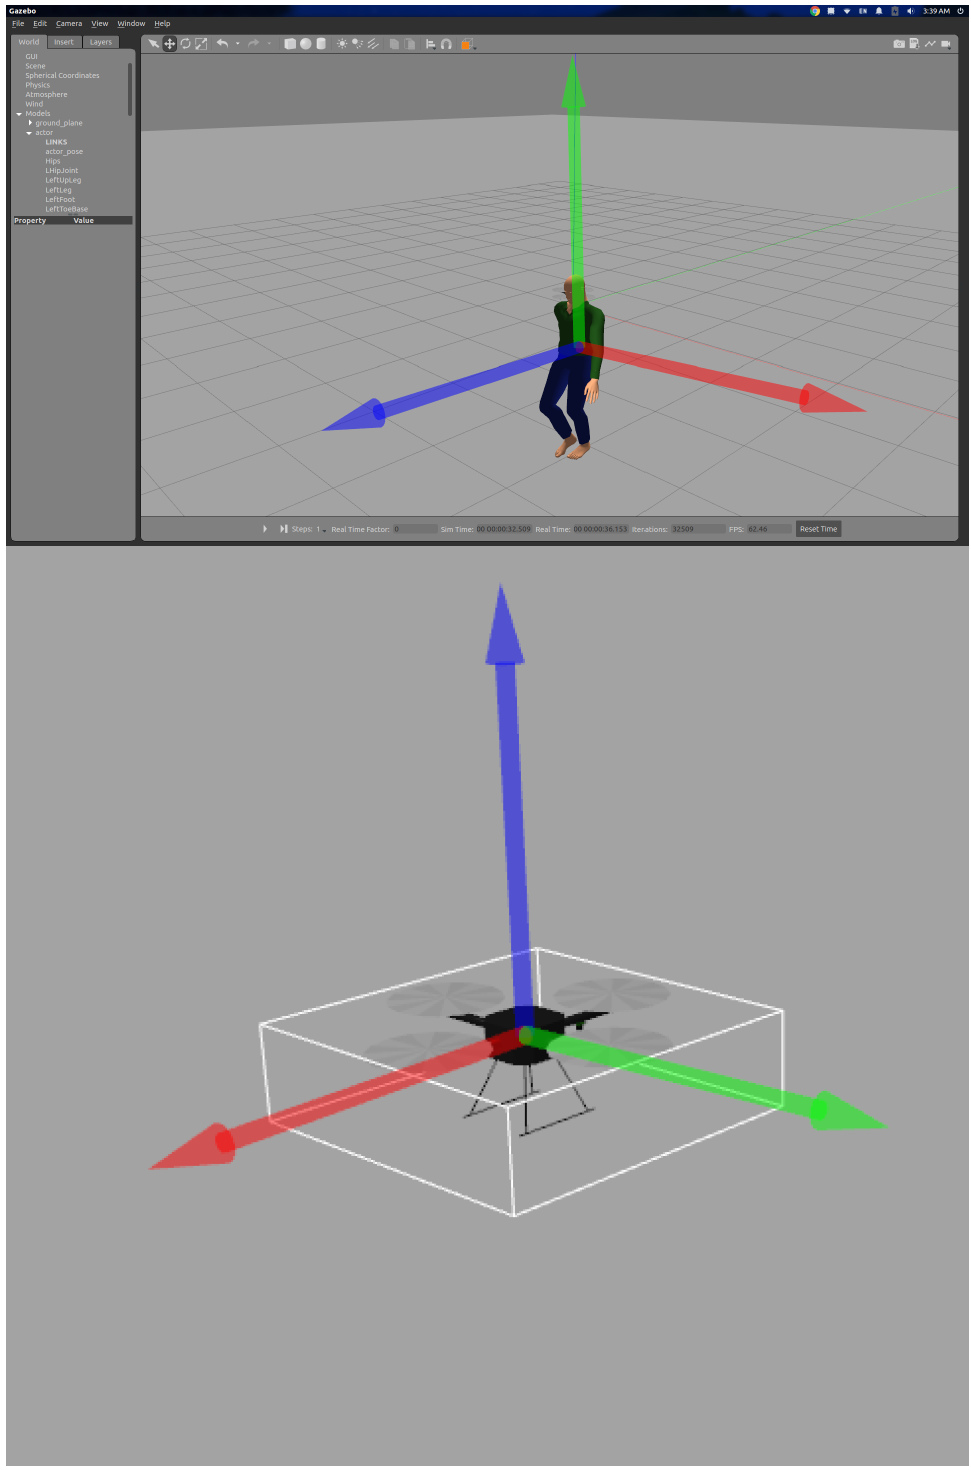
\includegraphics[width=9cm]{gazebo-models.PNG}
	\caption{Simulation models of quadrotor and human subject\label{Simulation}}
\end{figure}

%\newpage
\section{Experiments and results}
\label{sec:Experiments and results}

\subsection{Experiments}
\label{sec:Experiments}

A gazebo simulation is used for all of the experiments. The simulation consists of a quadrotor and actor based on humans moving on certain trajectories, which at the moment are fixed. The quadrotor used is \emph{hector-quadrotor} and for capturing images the onboard camera is used, the resolution of capture is 320x240. Now, the reason methods discussed before works, which are based on feature point detection, is when testing for detection of ORB features on the obtained image we got 400 feature points.

Images captured are sent to GPU server on which a tensorflow API is used to perform detection using SSD, this is done to simulate the real world implementation of the
pipeline. The frequency of the camera was set to 15Hz as the fastest detection was being done at 14Hz and feeding in more frames would only consume bandwidth of the
connection used to transfer images between the GPU server and simulation.

Support was added for more complex trajectories of the human subject such as moving in a square and with varying speeds and turn rates. This allows the simulation
to better model real world scenario. Also, this increased a challenge for quadrotor since the subject no longer permanently stayed inside the camera field of view. This also helped avoid local optima states for the quadrotor where it could keep the subject at center by just changing the yaw values.

Depth estimation portions were worked upon both in using stereo camera as well as monocular version, since the previous method of estimating the distance by the
area of the bounding box was unreliable. The area based estimate changed quadratically with distance, voiding the linear requirement of the simple control, as well as changed drastically in case of occlusion or if the human subject was
at an edge of the frame.

Kalman filter was implemented for high rate control input generation as well as occlusion avoidance. This helped take care of the issue of missing detections in hard-to-detect frames as well as smoothed out the detections, aiding in easier control. It also provided an added functionality of ability to incorporate occlusion/ out-of-frame cases.

Tracking node was developed for object detection in crowded environments. KCF was incorporated into the pipeline along with kalman filter to provide better estimates since it also uses information directly from the frames unlike kalman filter. This provided an added functionality of ability to incorporate cases with multiple moving subjects.

\begin{figure}[htb]
	\centering
	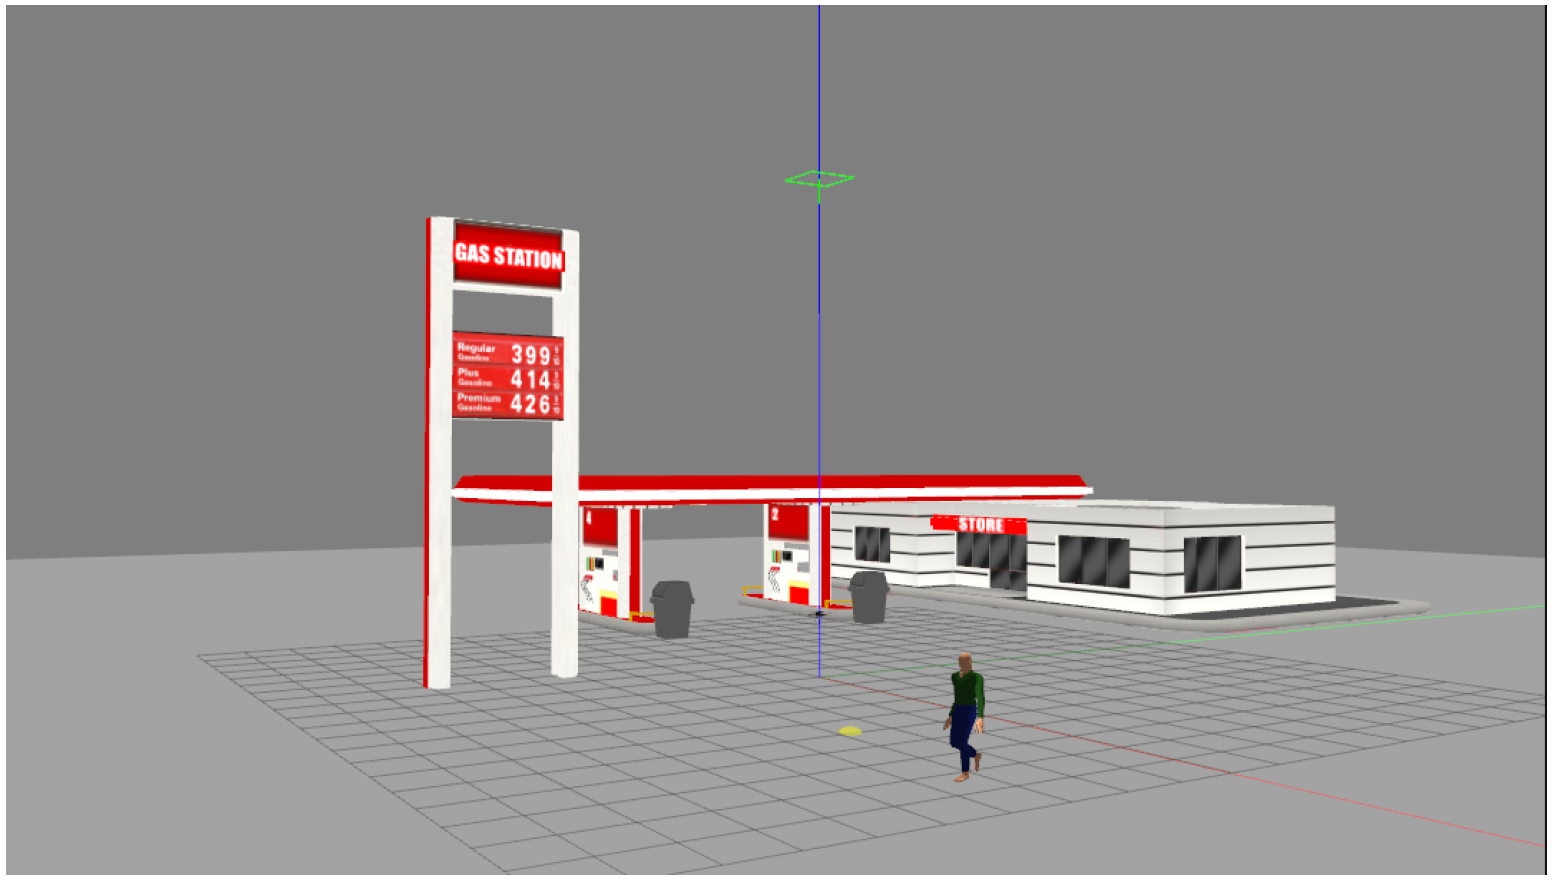
\includegraphics[width=15cm]{gazebo-setup.PNG}
	\caption{Experimental setup in Gazebo\label{Experimental setup in Gazebo}}
\end{figure}

\subsection{Specifications}
\emph{Quadrotor specifications:}
	Hector quadrotor gazebo model
	\newline Inertial Mass Value: 1.477 units
	\newline Onboard sensors(for implementation on a real quadrotor):
	\vspace{-5mm}
	\begin{itemize}
		\item 3 x gyroscopes
		\vspace{-5mm}
		\item 3D accelerometer \vspace{-5mm}
		\item 3D magnetometer \vspace{-5mm}
		\item Vertical distance (ultrasound), 16.66 Hz sample rate \vspace{-5mm}
		\item Power: LiPo batteries, 6 cells, 22.2 V, 222.0 Wh, 10000 mAh
	\end{itemize}	
	 
	\noindent Base Station capabilities(for implementation on real quadrotor) :
	
	\begin{itemize}
		\item WiFi connectivity: 2.4 GHz and 5.0 GHz spectra,  100Mbps, TCP/IP support \vspace{-5mm}
		\vspace{-5mm}\item Other connectivity: 3G, (2100/850/900 MHz), 4G LTE
	\end{itemize}
		
\noindent\emph{Mounted camera specifications:}
	Generic stereo camera \vspace{-5mm}
	\begin{itemize}
		\item Update rate: 30 Hz \vspace{-5mm}
		\item Resolution: 400 x 400 \vspace{-5mm}
		\item Image format: RGB \vspace{-5mm}
		\item Horizontal field of view: 80$^{\circ}$ 
	\end{itemize}
	
%\clearpage
\emph{Processing time and requirements for image transfer, detection:}

\begin{table}[h]
	\centering
	\begin{tabular}{| c | c | c | c | c |}
		\hline
		Devices	& Image capture & Detection	& Uncompressed transfer & Compressed	\\ \hline  \hline
		Intel i5-3250, No-GPU		& 34ms	& 130 ms	& NA	& NA\\ \hline
		Nvidia GeForce 960M	& 34ms	& 60ms	& NA	& NA\\ \hline
		Nvidia Titan X		& 34MS		& 5ms		& 500ms		& 10ms	\\ \hline
	\end{tabular}
	\caption{Time Analysis}
	\label{table:Time Analysis}
\end{table}

\emph{System requirements for running object detection node:}
	\begin{itemize}
		\item CUDA® Toolkit 8.0. \vspace{-5mm}
		\item The NVIDIA drivers associated with CUDA Toolkit 8.0. \vspace{-5mm}
		\item GPU card with CUDA Compute Capability 3.0 or higher. 
	\end{itemize}


\subsection{Results}
\label{sec:Results}

Detailed time based analysis can be obtained in Table 7.1 for various submodules in the pipeline.

\begin{figure}[htb]
	\centering
	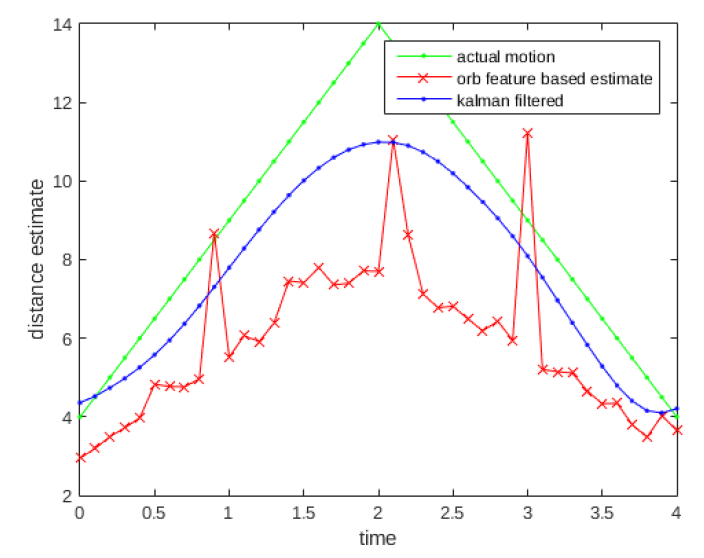
\includegraphics[width=12cm]{distance-estimate.PNG}
	\caption{Results of distance estimation by Kalman filter as
		well as orb feature method against ground truth\label{Result}}
\end{figure}

The results were recorded in rosbag files which are file formats for storing ROS message data. These subscribe to a certain specific topics and can also be played back to the same topics.The rosbag files are further changed into .mat files for working in MATLAB using a bagReader module available in MATLAB. Then the data is used for plotting the results in MATLAB graphs.

The corners of the human trajectory is made erratic to simulate the uncertain nature of human movement. The quadrotor is set to follow the human keeping different distance threshold to check the effectiveness at 3m, 5m, and 10m. The effect of varying height is also tested as the quadrotor is set at 1.5m, 3m and 5m above the ground. A different path with different velocity is also tested on.

\begin{figure}[htb]
	\centering
	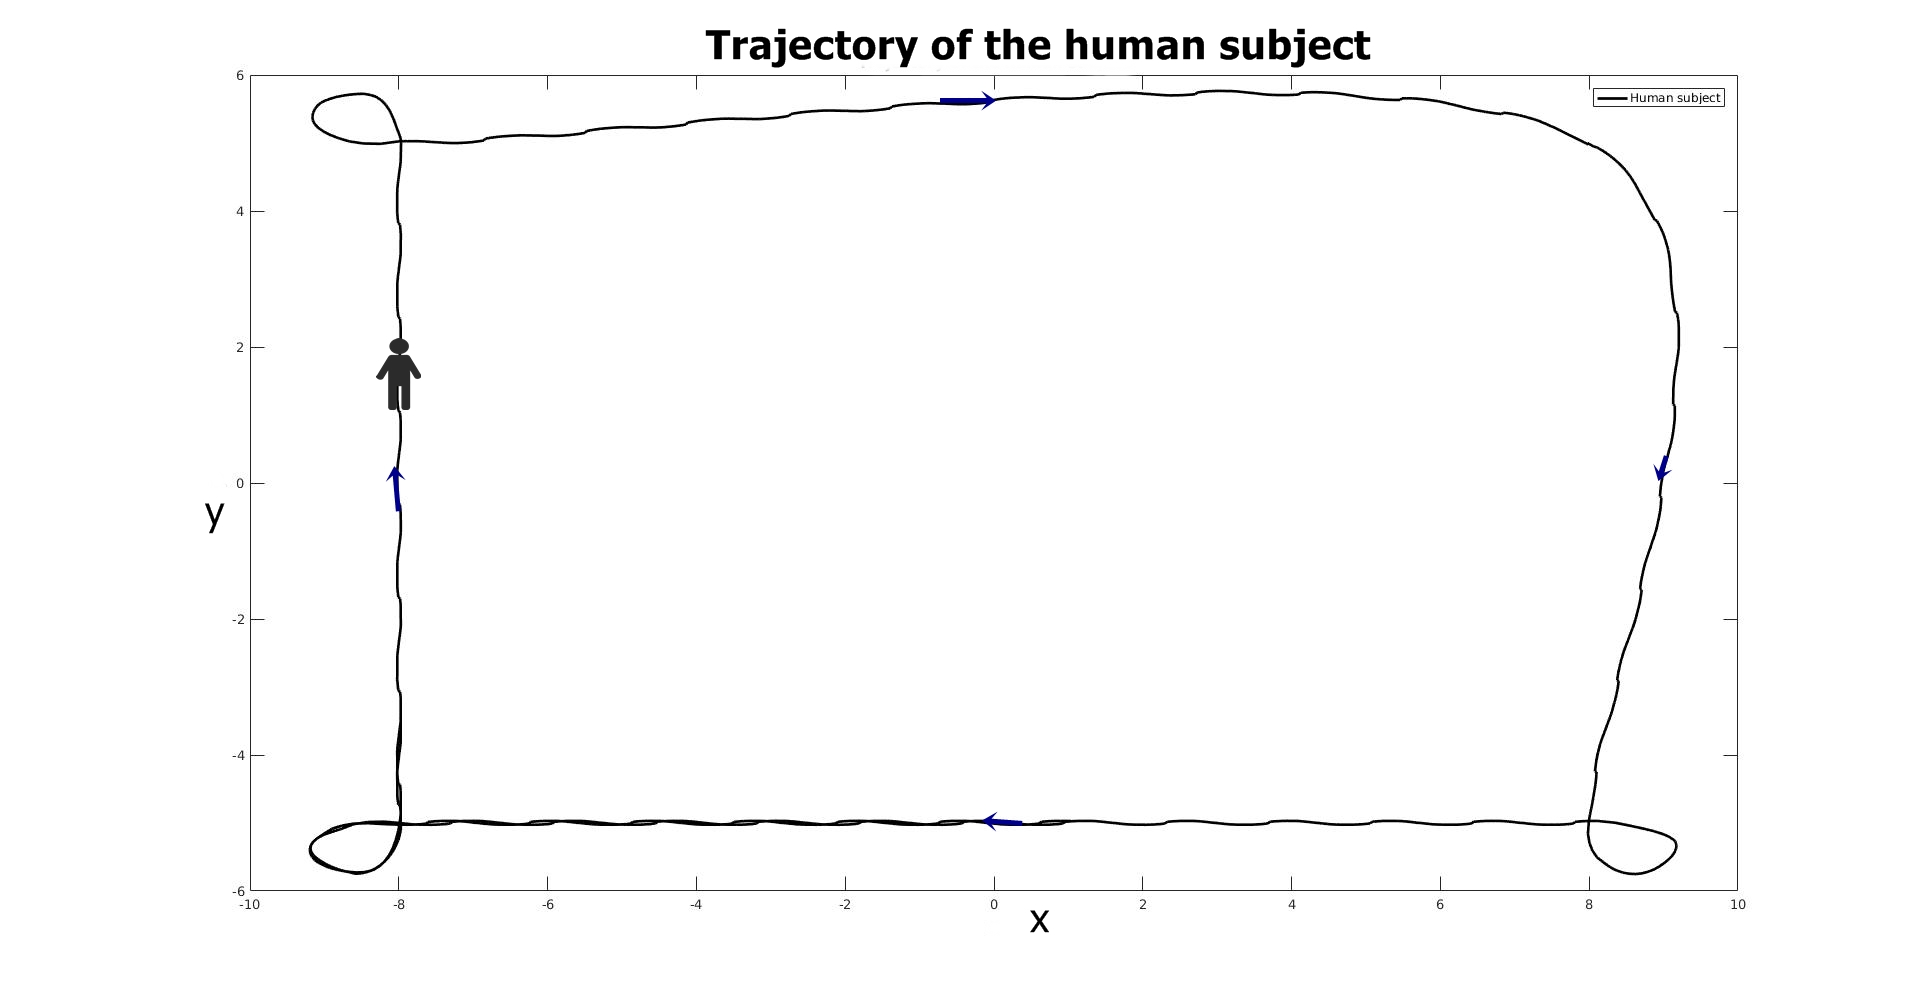
\includegraphics[width=15cm]{human_path2D.jpg}
	\caption{Trajectory of the human subject\label{Trajectory of the human subject}}
\end{figure}

\subsubsection{Results for 3m distance, 1.5m height}
The results shows the quadrotor starting from origin and aligning itself to follow the human subject trying to keep the distance required.

\begin{figure}[htb]
	\centering
	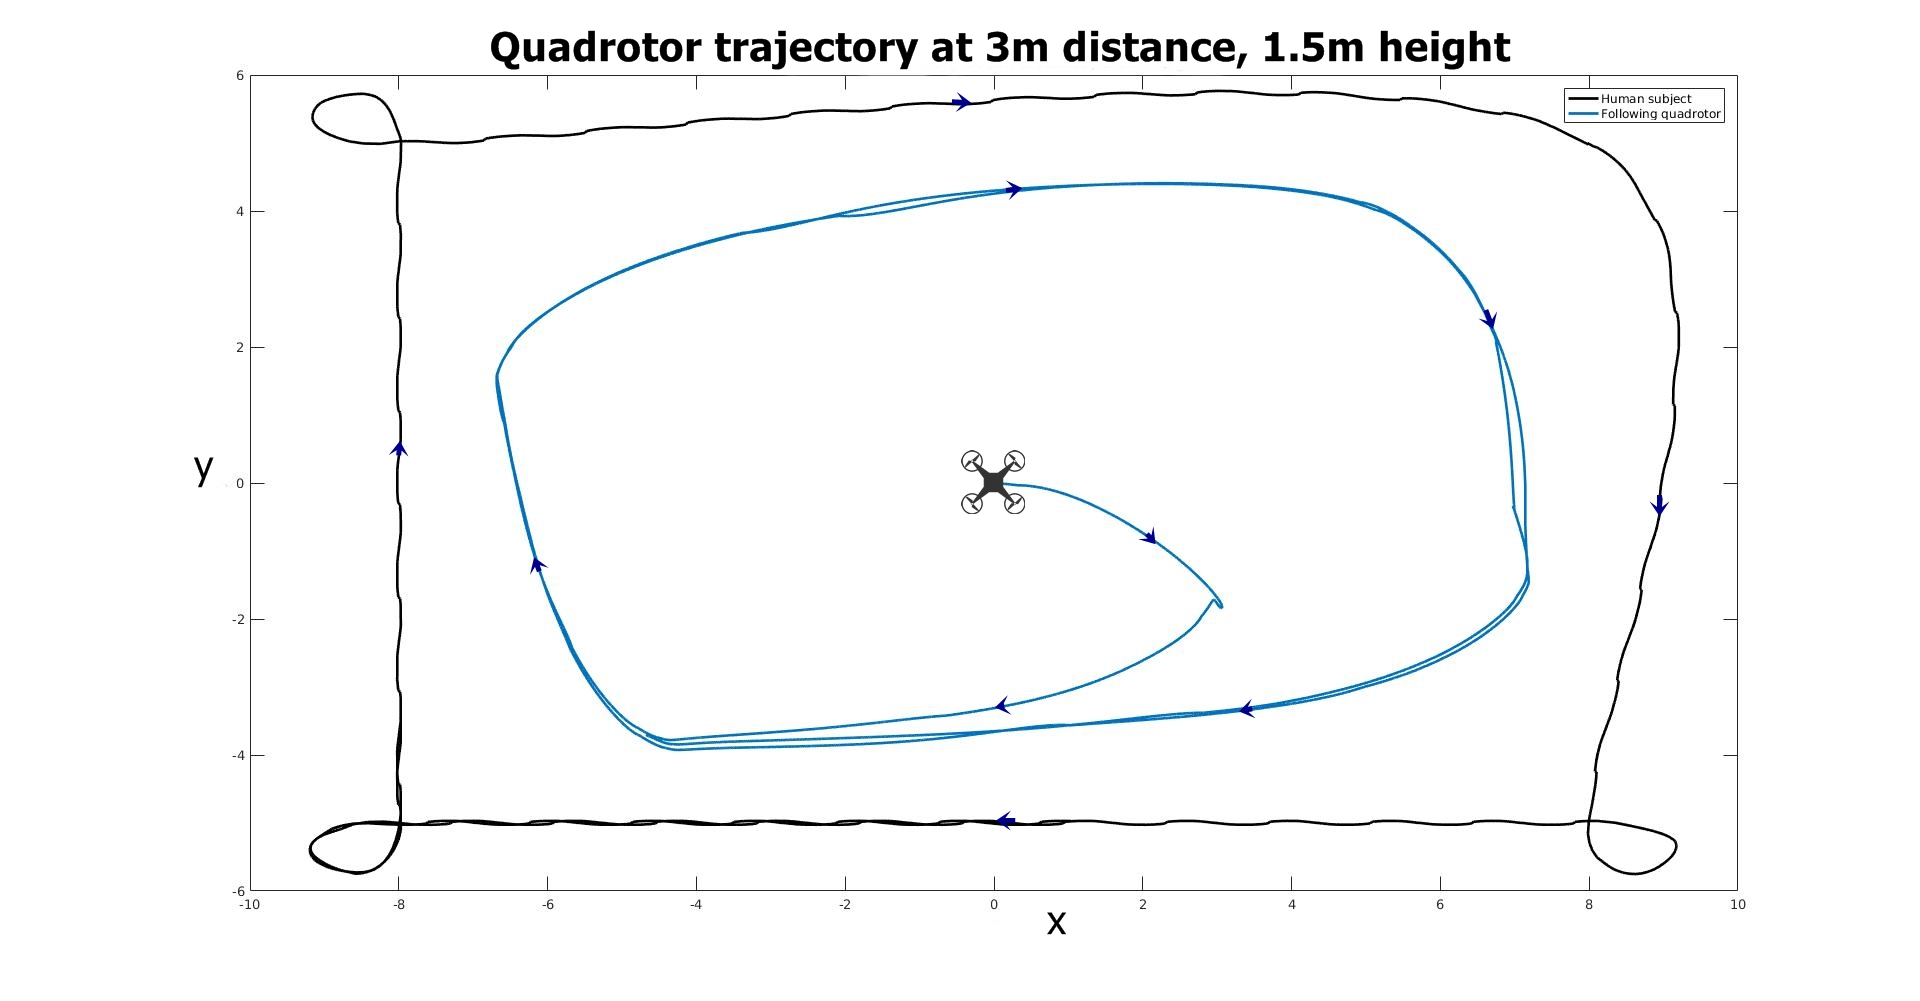
\includegraphics[width=15cm]{quad_path_for_3m.jpg}
	\caption{Quadrotor path for 3m distance, 1.5m height\label{Quadrotor path for 3m distance, 1.5m height}}
\end{figure}

The distance vs time graph shows the deviation in distance is around average of 3m.
\begin{figure}[htb]
	\centering
	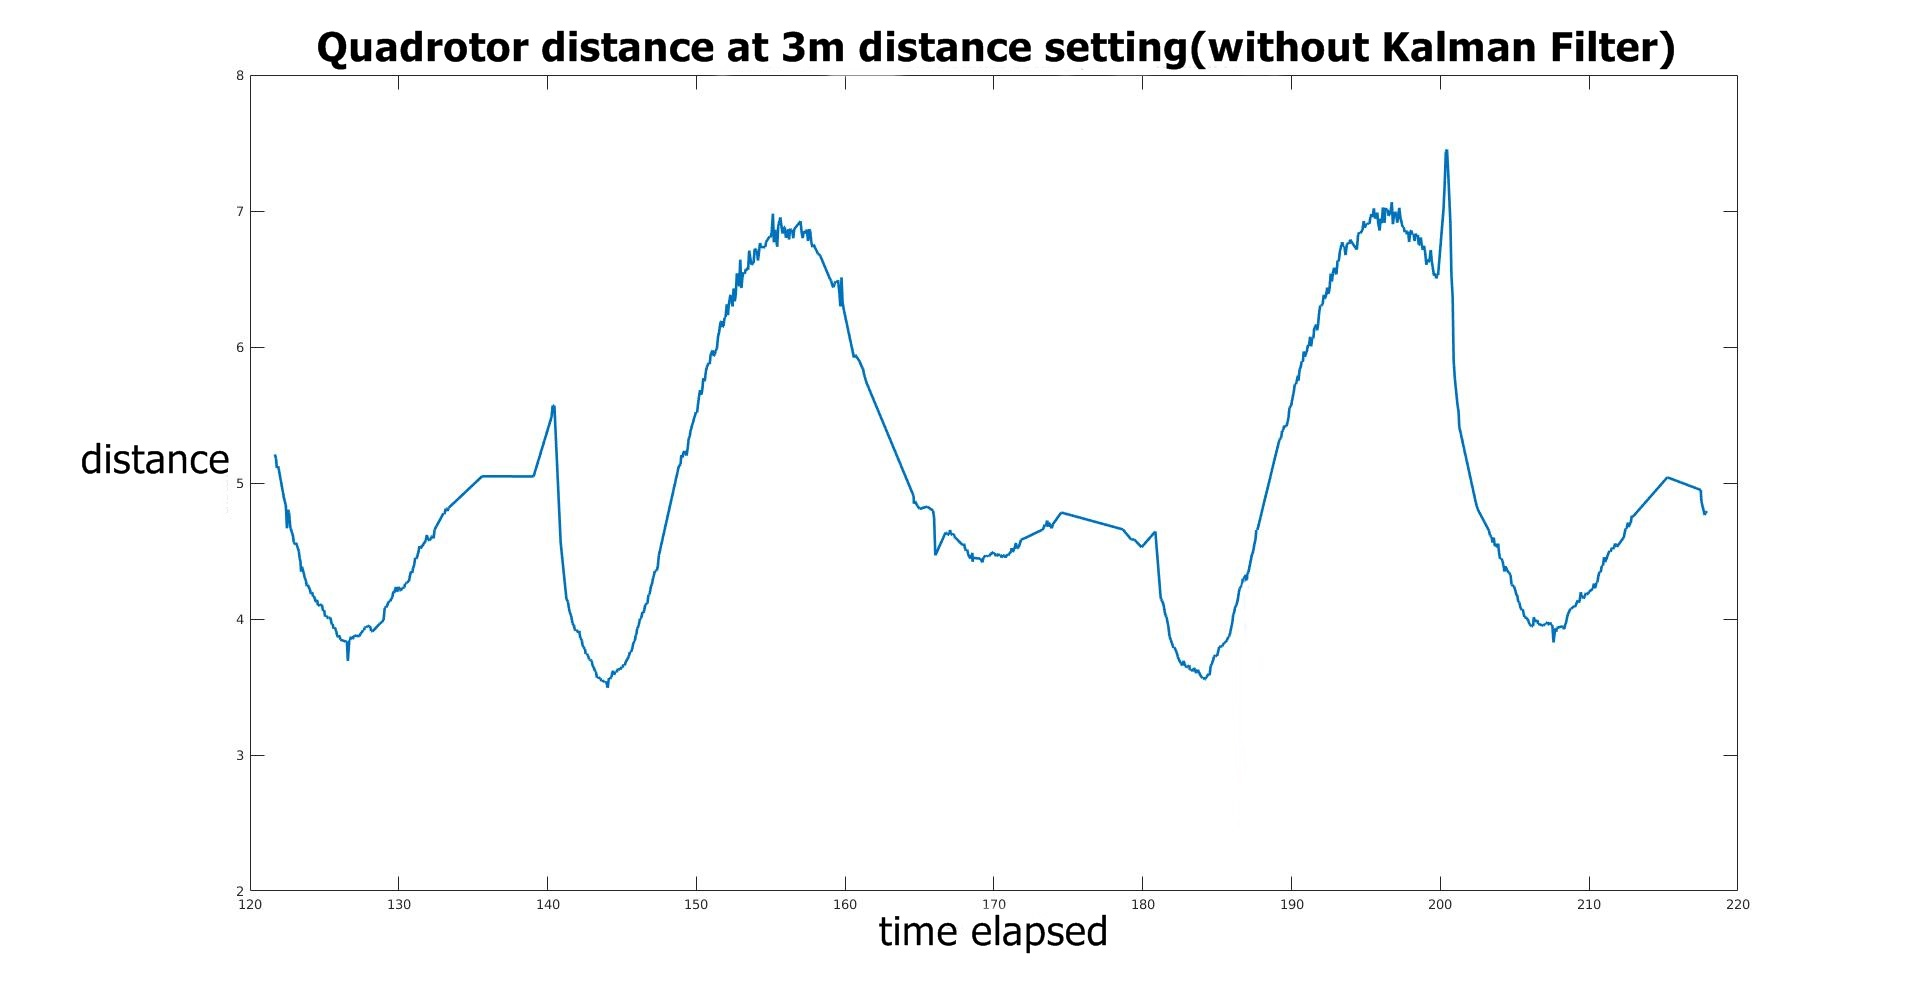
\includegraphics[width=15cm]{distance3m_wokf.jpg}
	\caption{Distance of quadrotor for 3m setting, 1.5m height\label{Distance of quadrotor for 3m setting, 1.5m height}}
\end{figure}

\subsubsection{Results for 5m distance, 1.5m height}
The result shows the quadrotor is able to effectively track the subject from a distance of 5m.

\begin{figure}[htb]
	\centering
	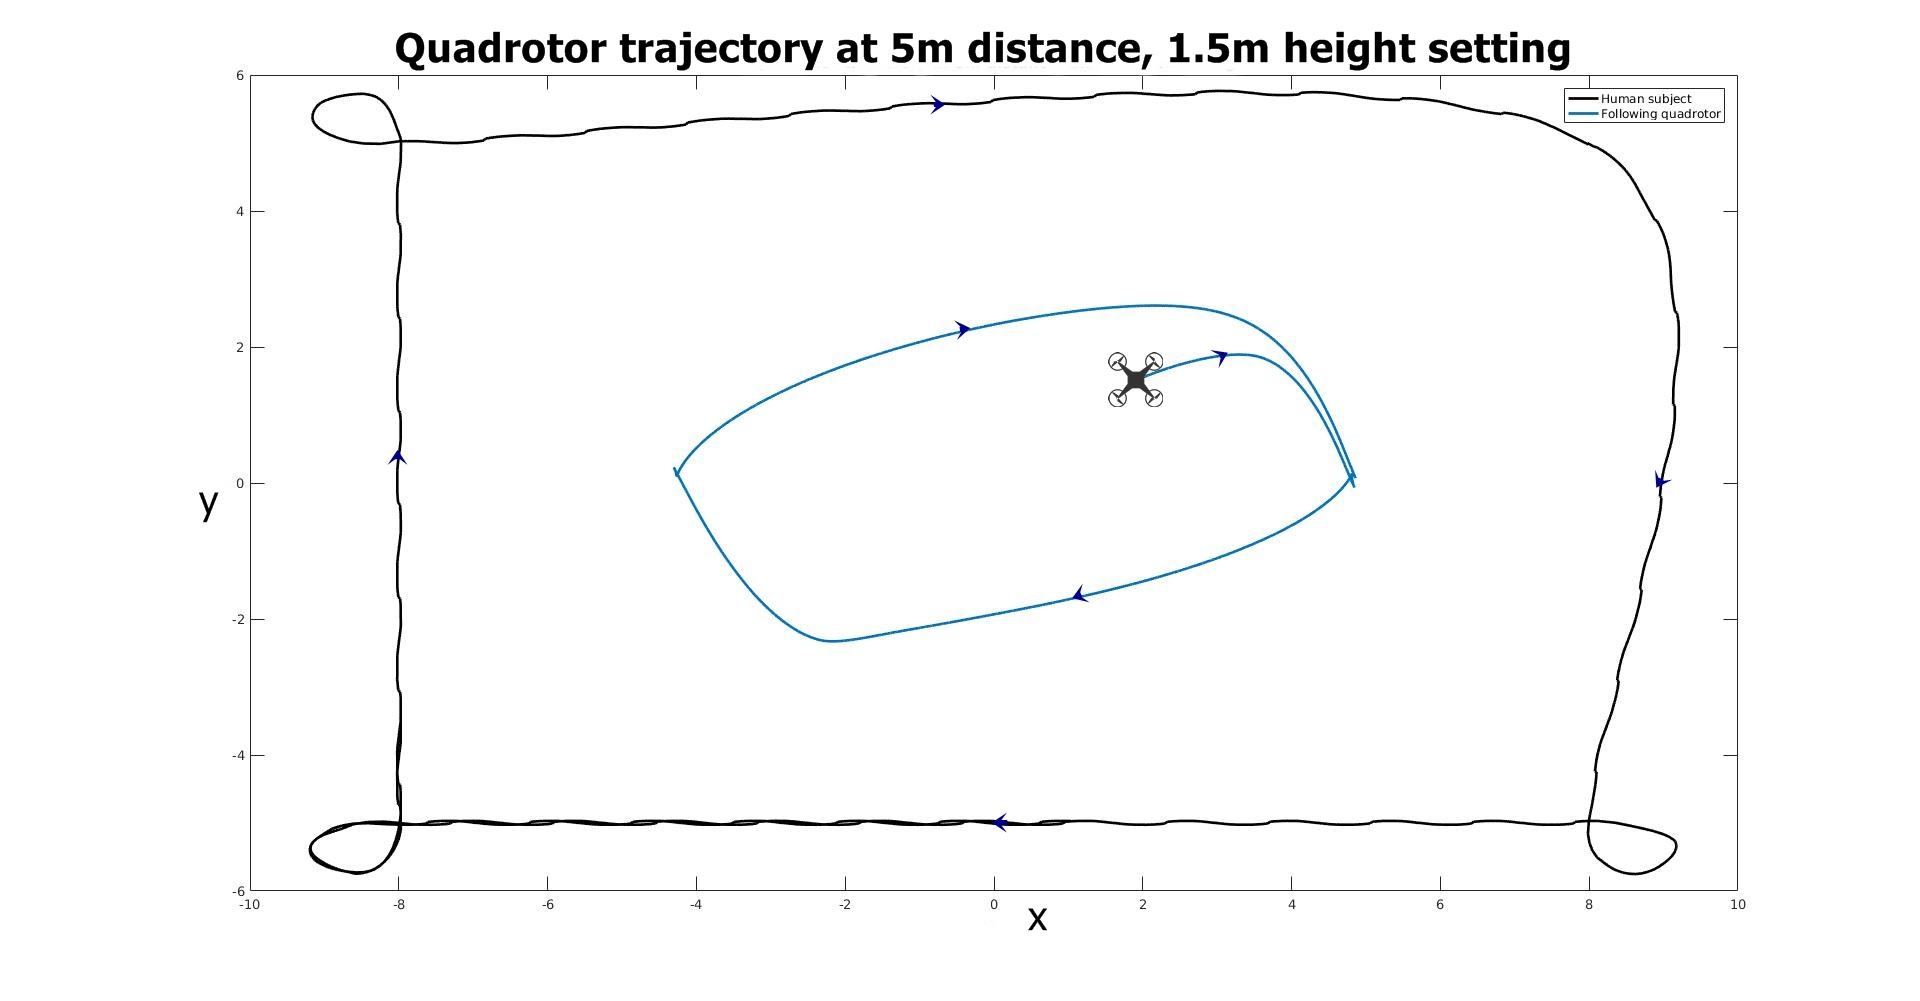
\includegraphics[width=15cm]{quad_path_5m.jpg}
	\caption{Quadrotor path for 5m distance, 1.5m height\label{Quadrotor path for 5m distance, 1.5m height}}
\end{figure}

The distance vs time graph shows the deviation from the set point for distance is at an average of 3m without applying kalman filter. 
\begin{figure}[!htb]
	\centering
	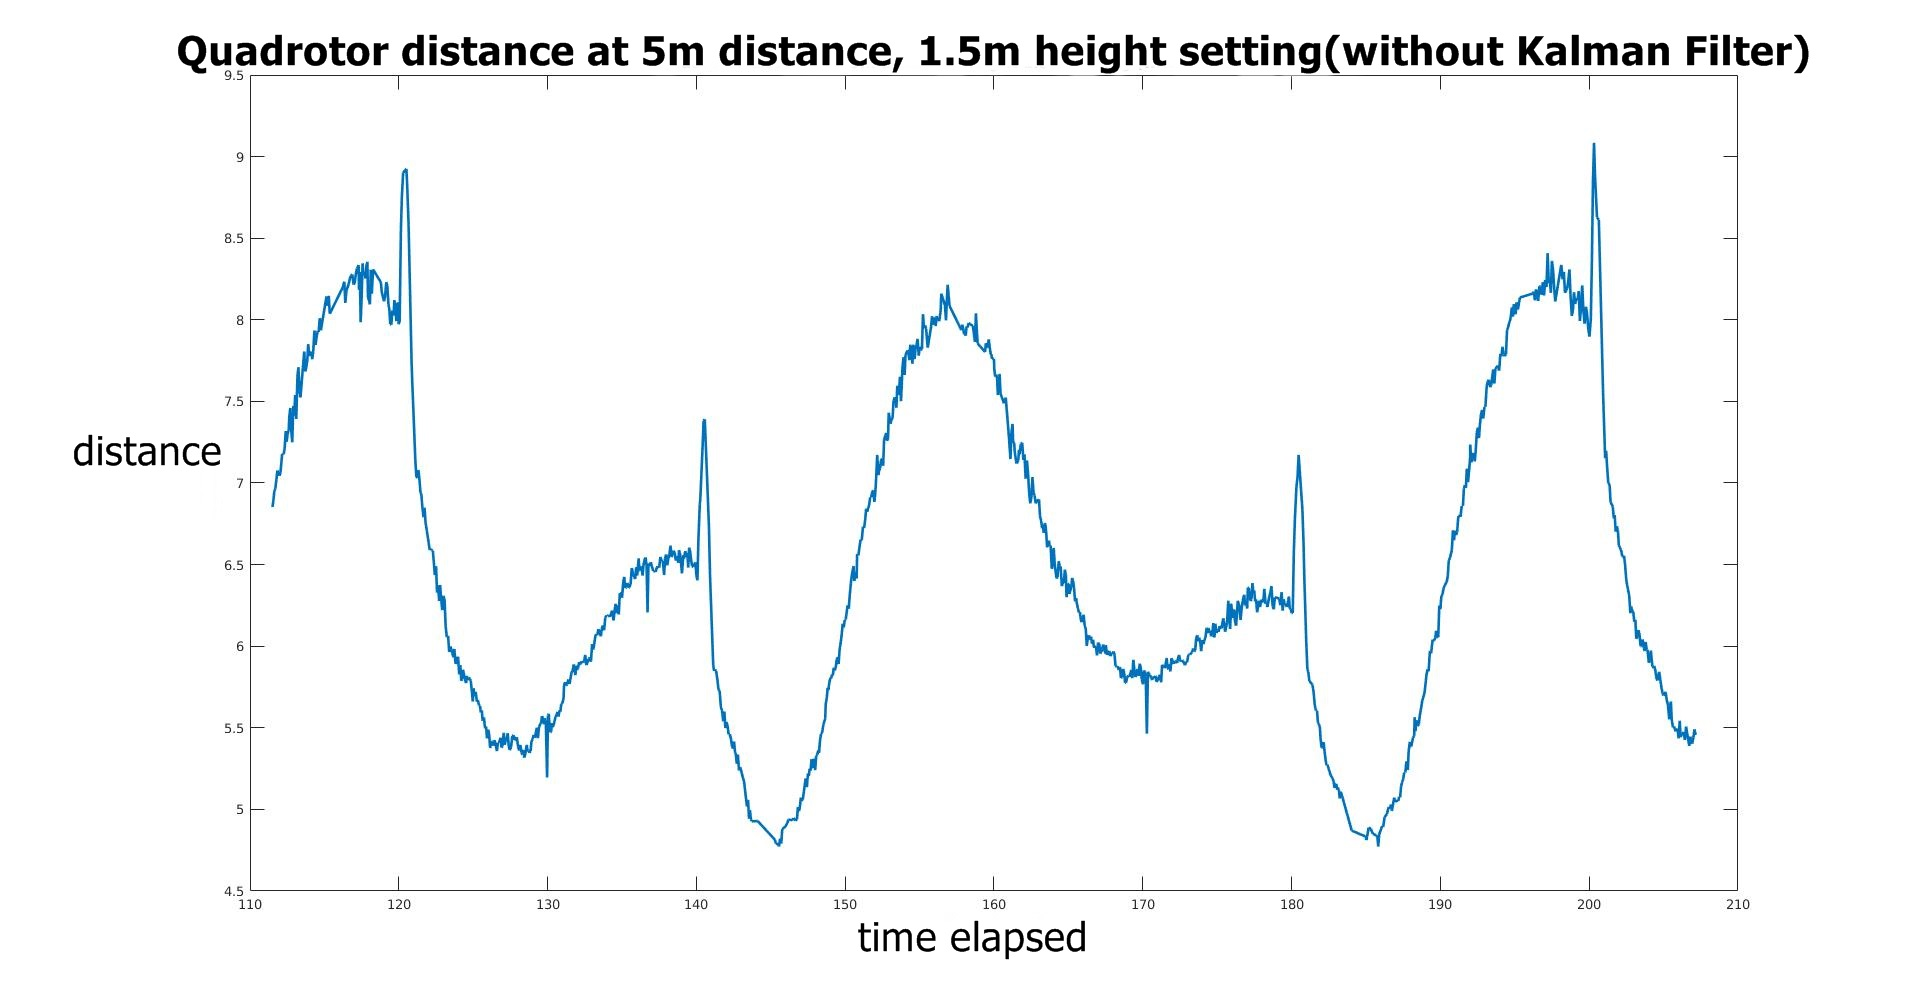
\includegraphics[width=15cm]{distance5m_wokf.jpg}
	\caption{Distance of quadrotor for 5m setting, 1.5m height, without Kalman filter\label{Distance of quadrotor for 5m setting, 1.5m height, without Kalman filter}}
\end{figure}
\newpage
While on using Kalman filter, the movement of the quadrotor is smoothed out, and also the average deviation from the set distance is reduced.
\begin{figure}[!htb]
	\centering
	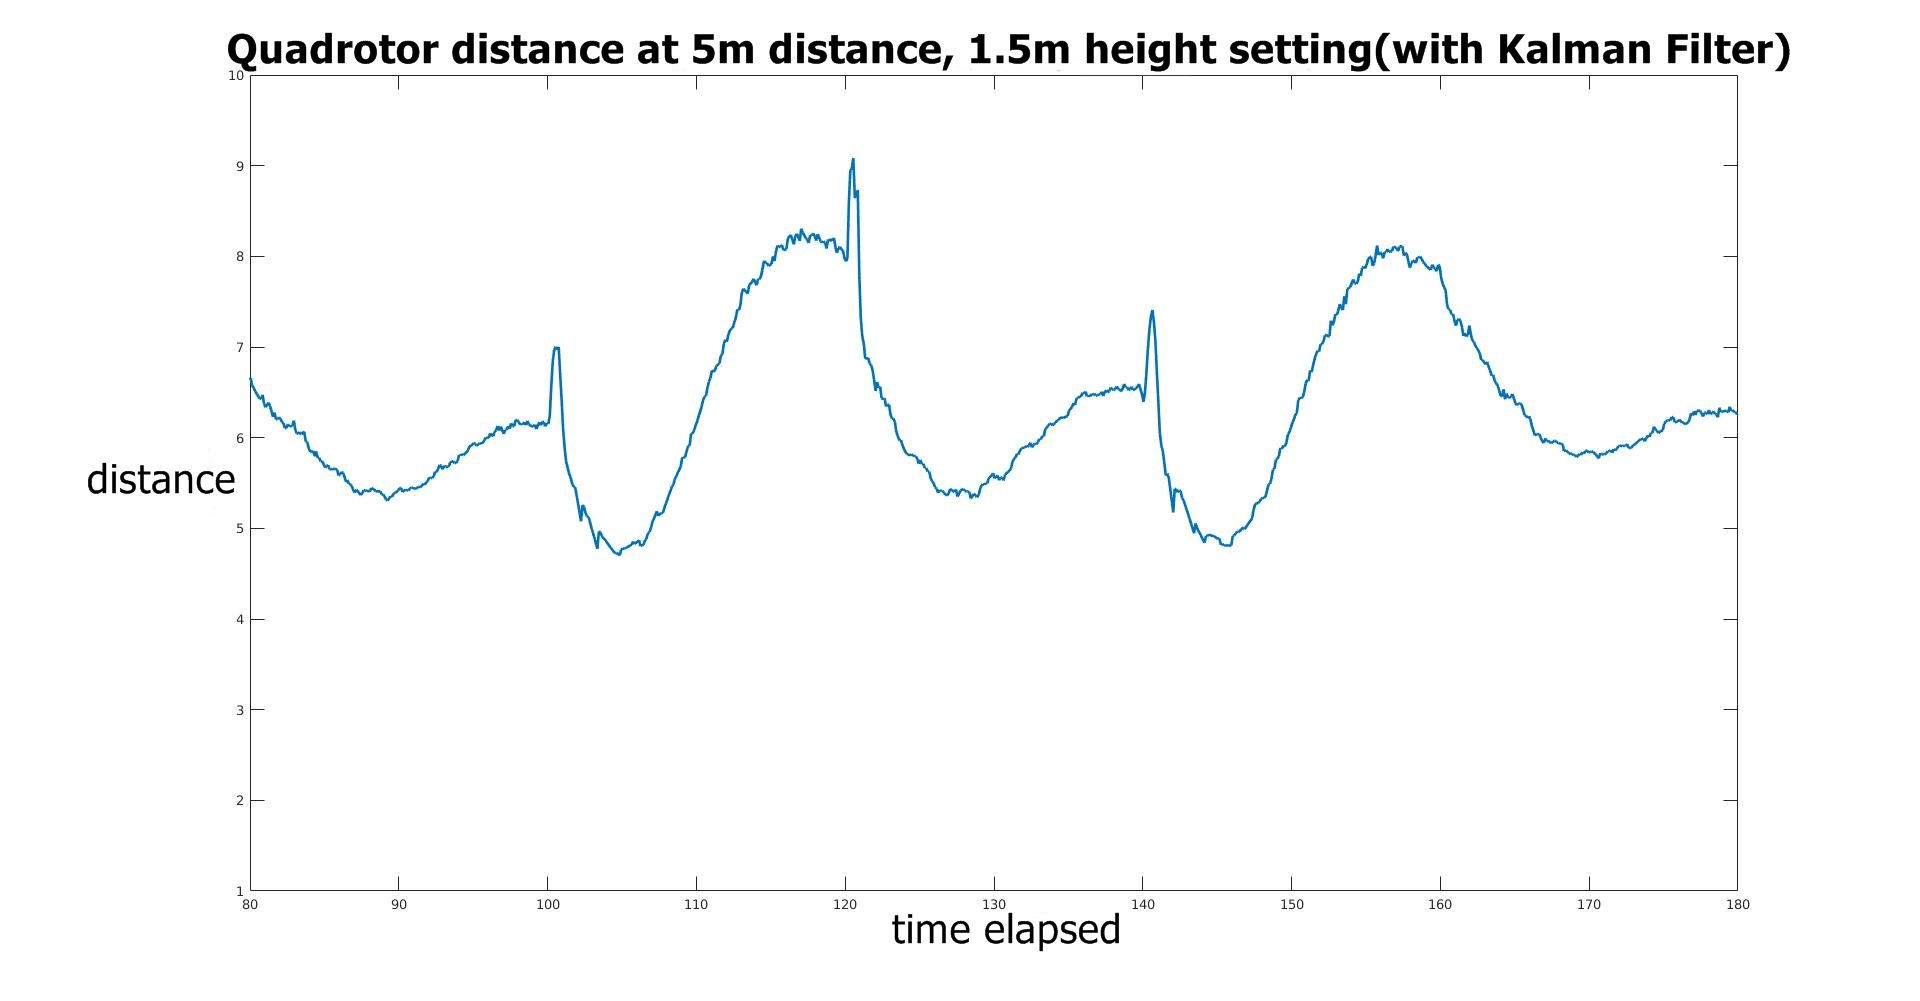
\includegraphics[width=15cm]{distance5m_wkf.jpg}
	\caption{Distance of quadrotor for 5m setting, 1.5m height, with Kalman filter\label{Distance of quadrotor for 5m setting, 1.5m height, with Kalman filter}}
\end{figure}

Following graph shows the midpoints of the detected bounding box along the whole time the quadrotor takes to complete the trajectory. The cluster of points shows that deviation in x and y direction is 30 and 20 pixels respectively, which is quite small.
\begin{figure}[!htb]
	\centering
	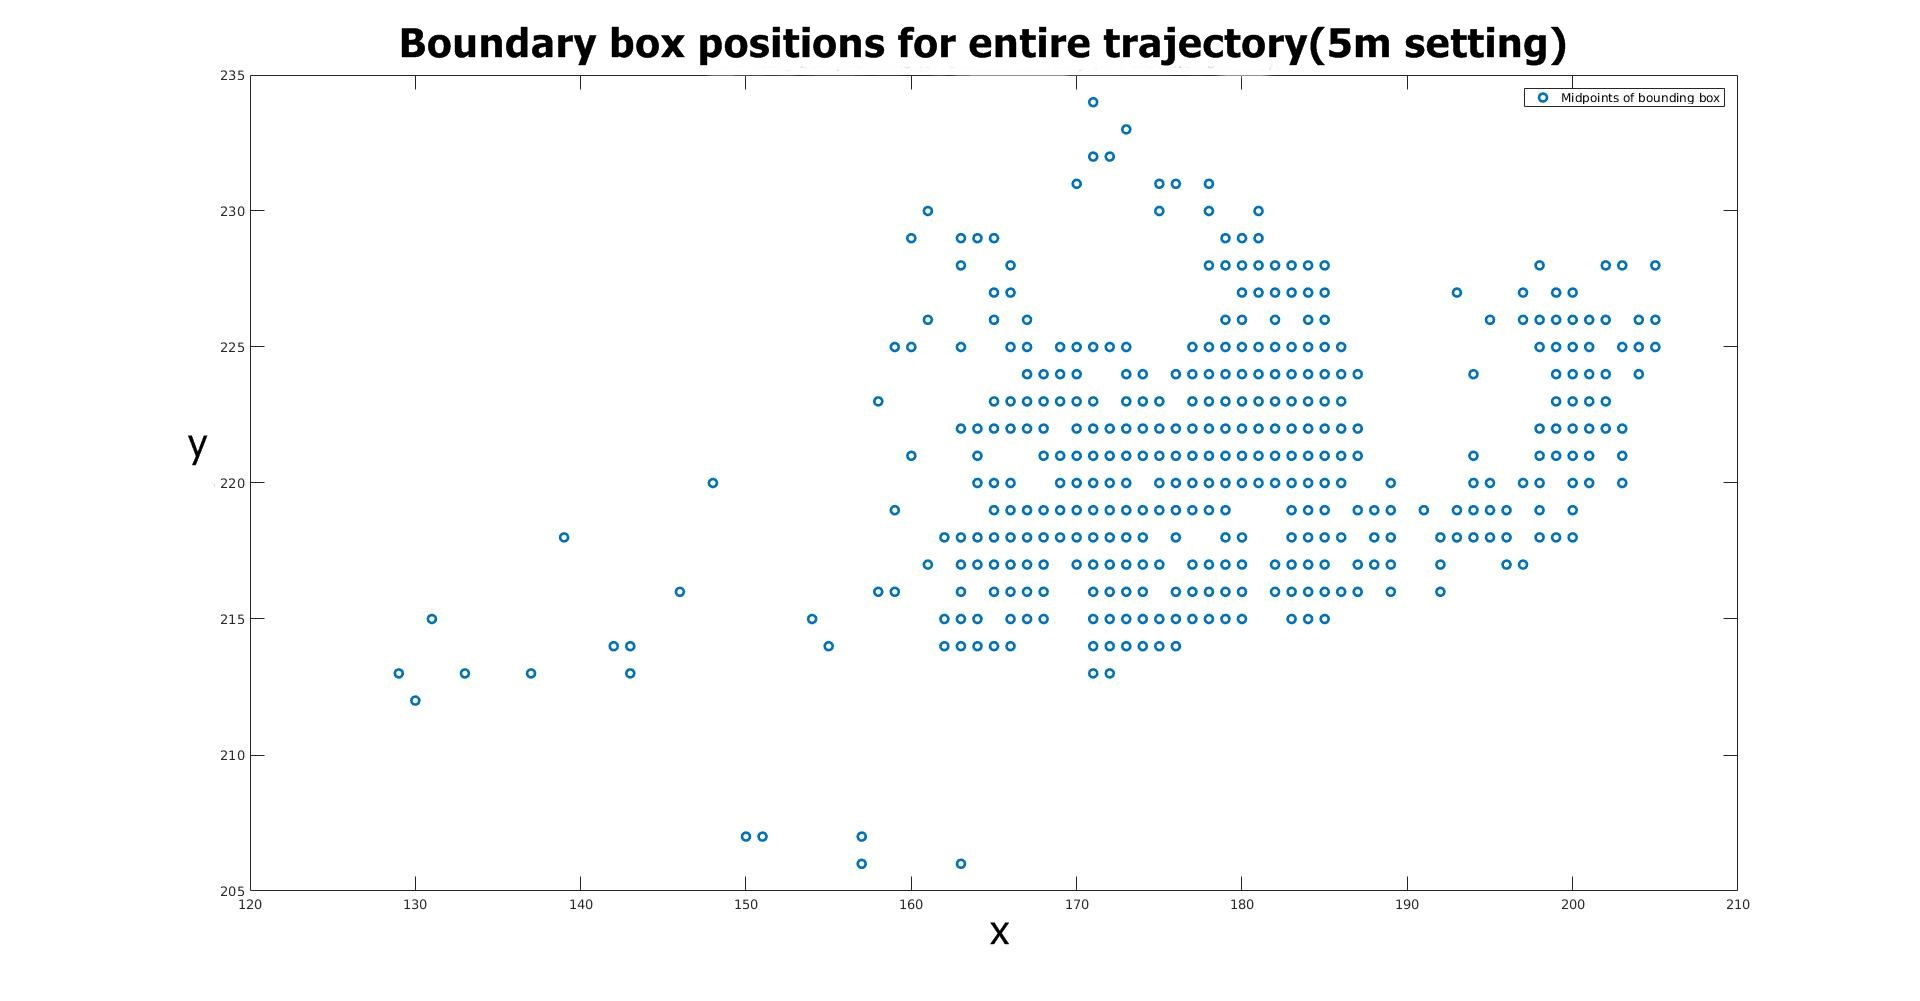
\includegraphics[width=15cm]{bounding_box_positions_5m_distance.jpg}
	\caption{Bounding box positions for 5m distance, 1.5m height\label{Bounding box positions for 5m distance, 1.5m height}}
\end{figure}

The confidence vs time graph shows the confidence level lies between 0.5 to 0.9. So the prediction is very much accurate about detecting human subject.
\begin{figure}[!htb]
	\centering
	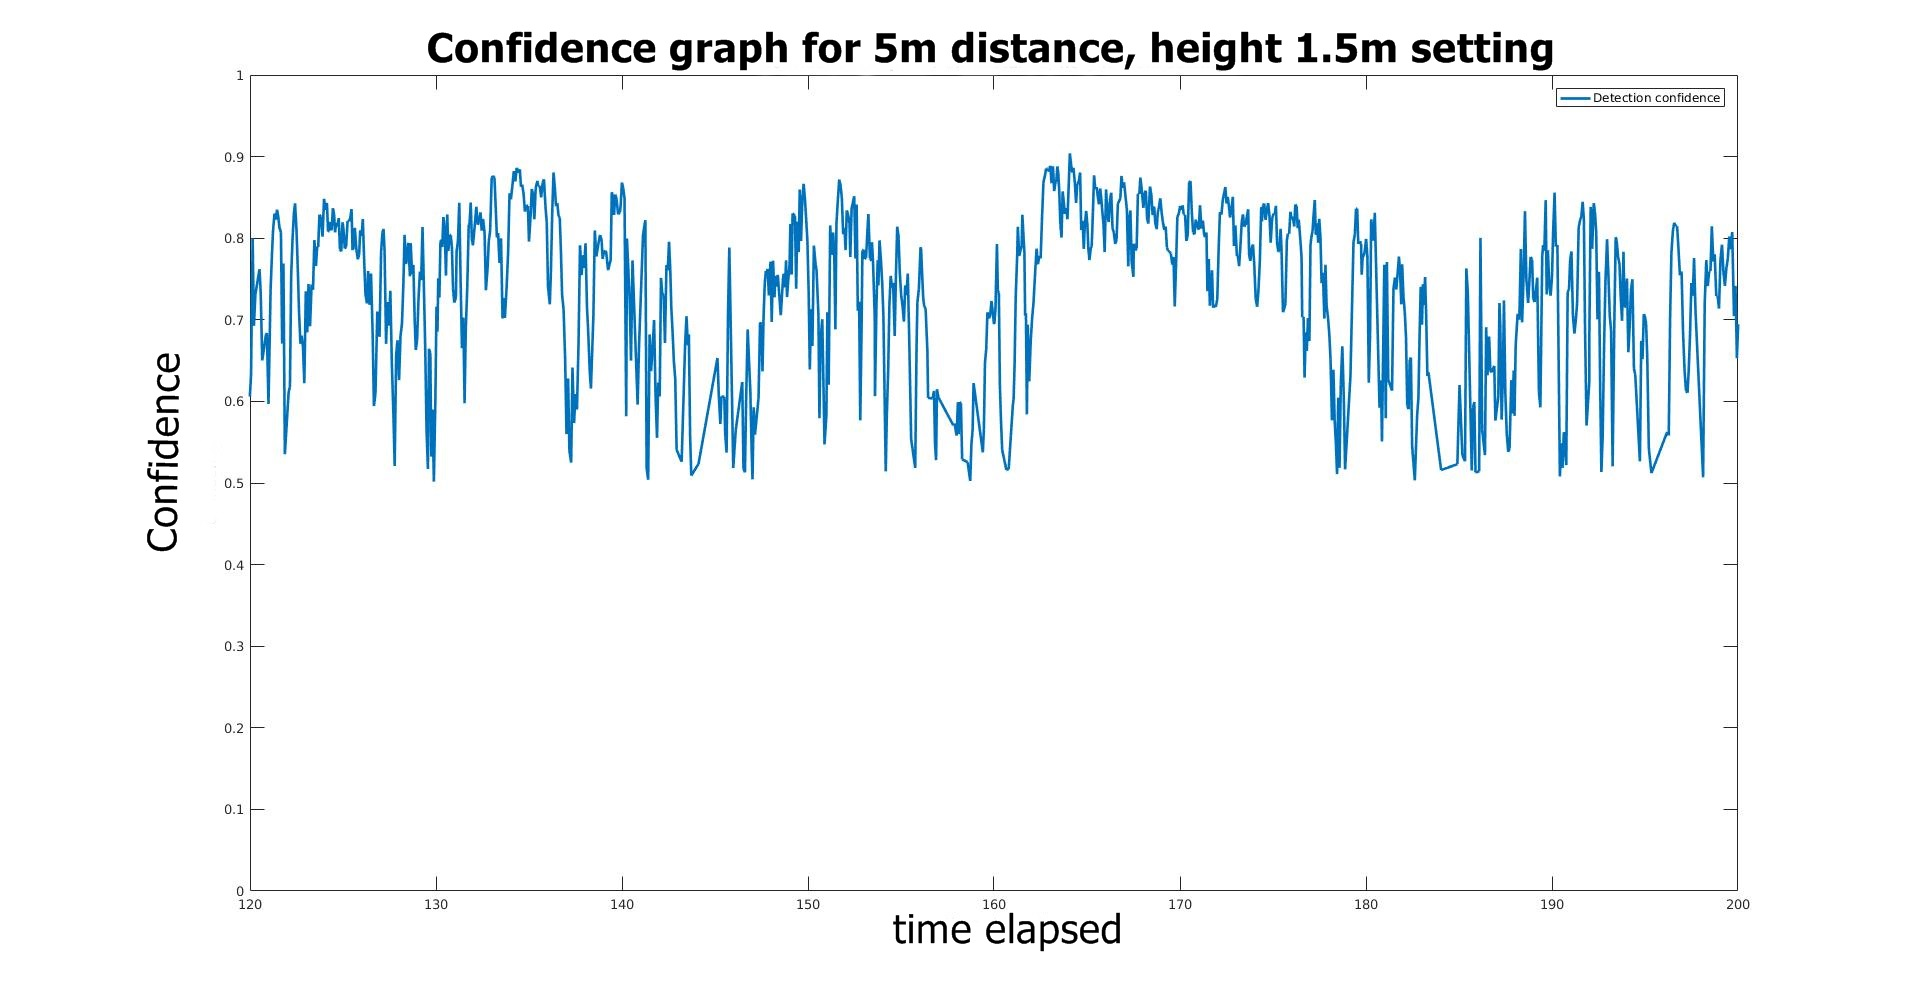
\includegraphics[width=15cm]{confidence_graph_d5m.jpg}
	\caption{Confidence graph for 5m distance, 1.5m height\label{Confidence graph for 5m distance, 1.5m height}}
\end{figure}

\newpage
\subsubsection{Results for 5m distance, 3m height}
The graphs show that the change in height has very negligible effect on the tracked path followed by the quadrotor.

\begin{figure}[!htb]
	\centering
	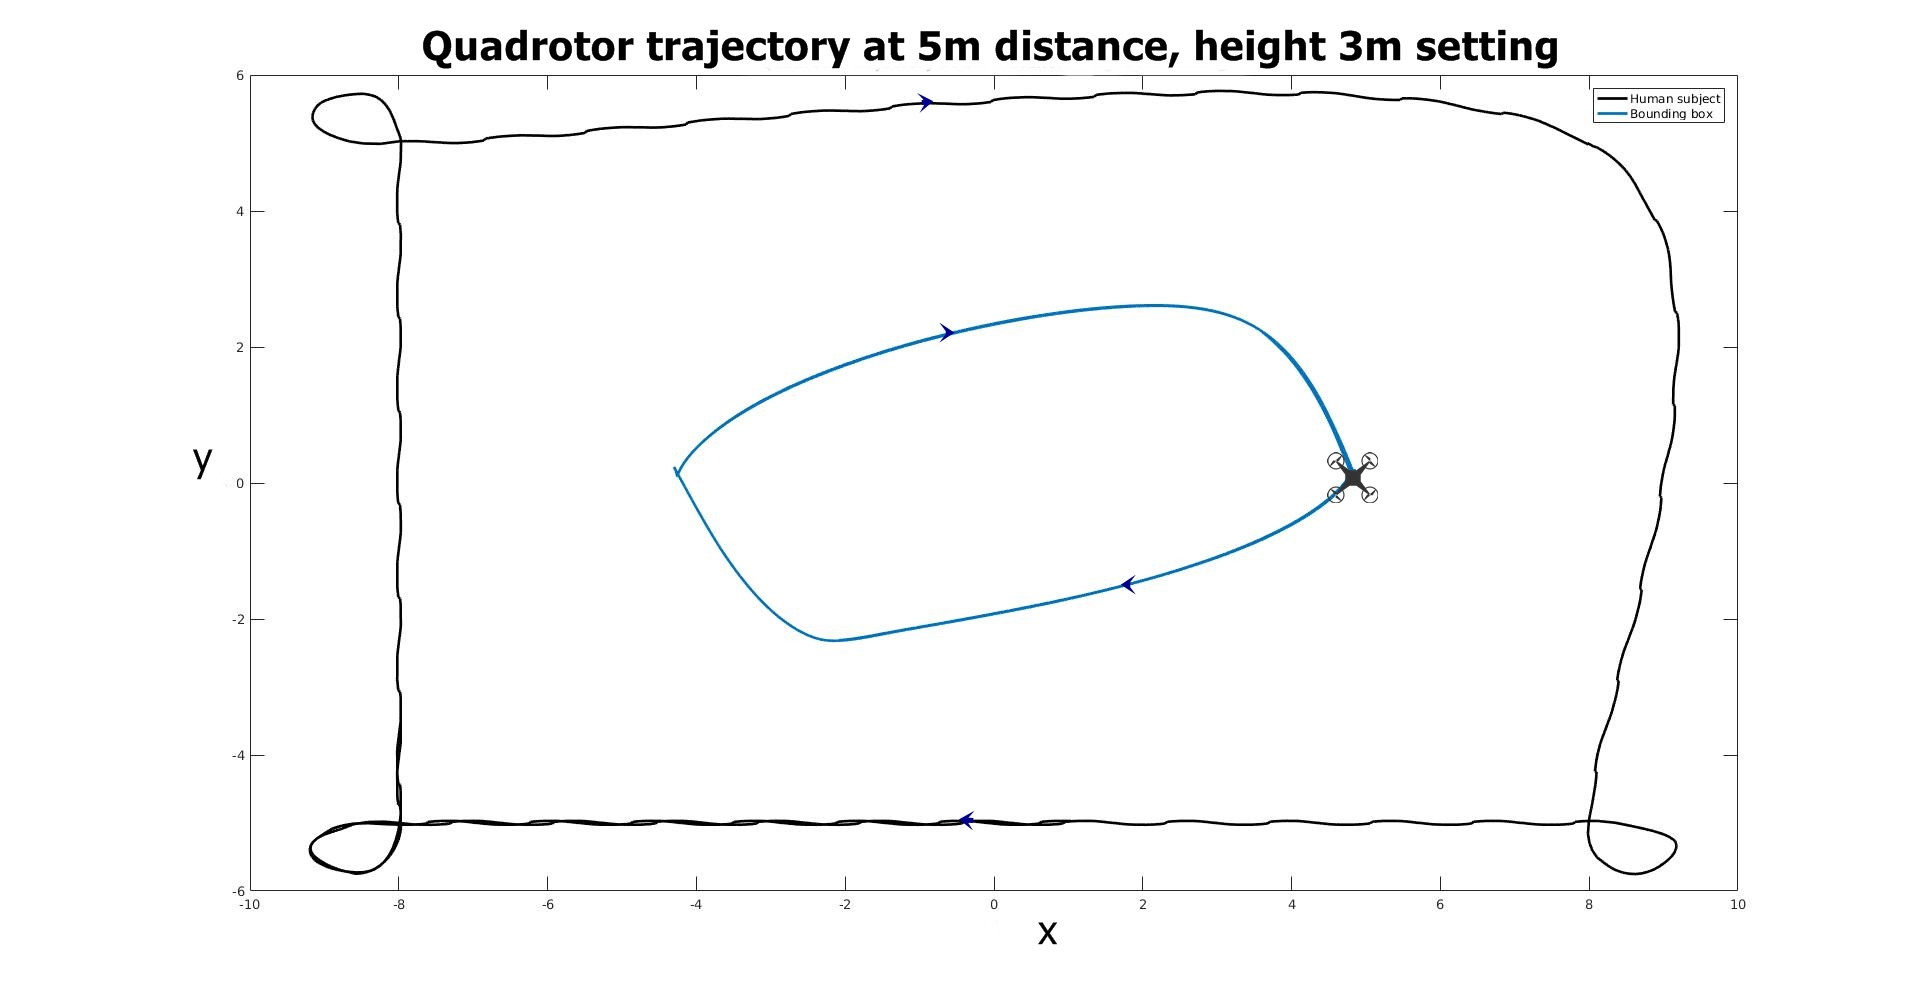
\includegraphics[width=15cm]{quad_path_3m_height.jpg}
	\caption{Quadrotor path for 5m distance, 3m height\label{Quadrotor path for 5m distance, 3m height}}
\end{figure}

The distance vs time graph shows the deviation from the set point for distance is at an average of 3m.
\begin{figure}[!htb]
	\centering
	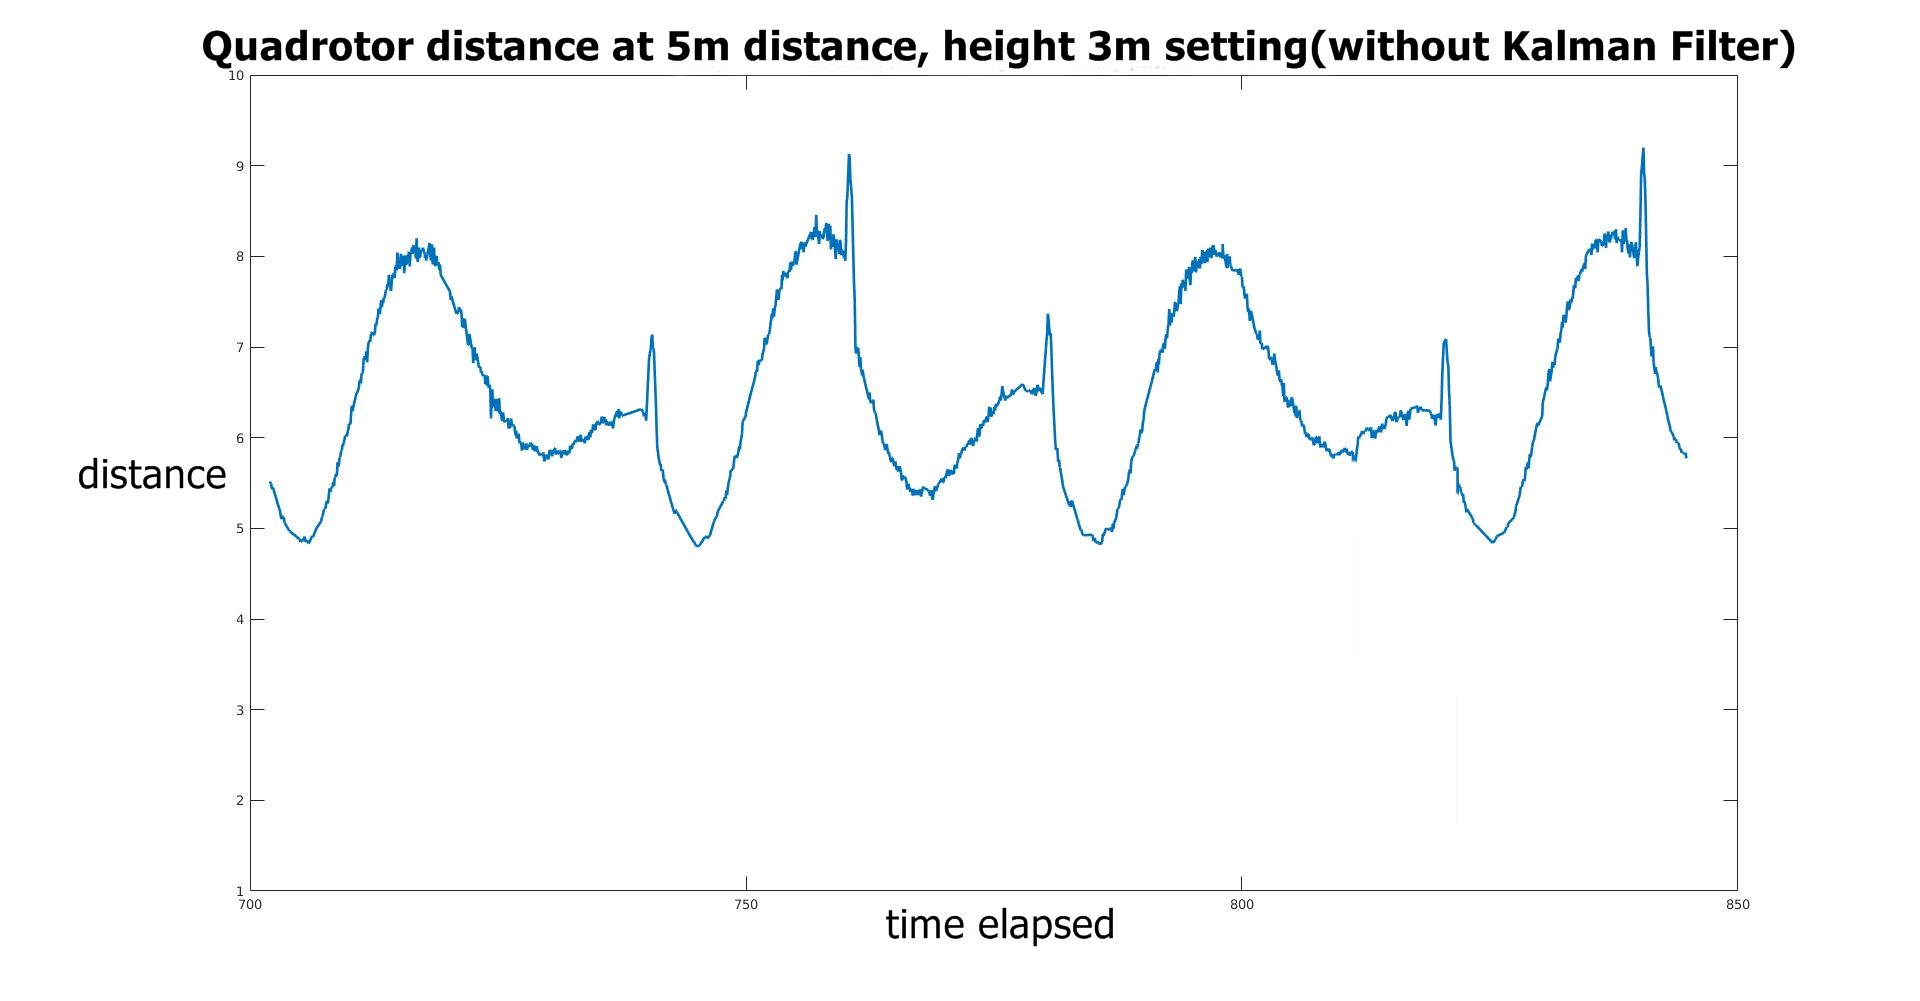
\includegraphics[width=15cm]{distance5m_height3m_wokf.jpg}
	\caption{Distance of quadrotor at 5m distance, 3m height\label{Distance of quadrotor at 5m distance, 3m height}}
\end{figure}

The cluster of points shows that deviation in x and y direction is 30 and 20 pixels respectively, which is similar to previous case.
\begin{figure}[!htb]
	\centering
	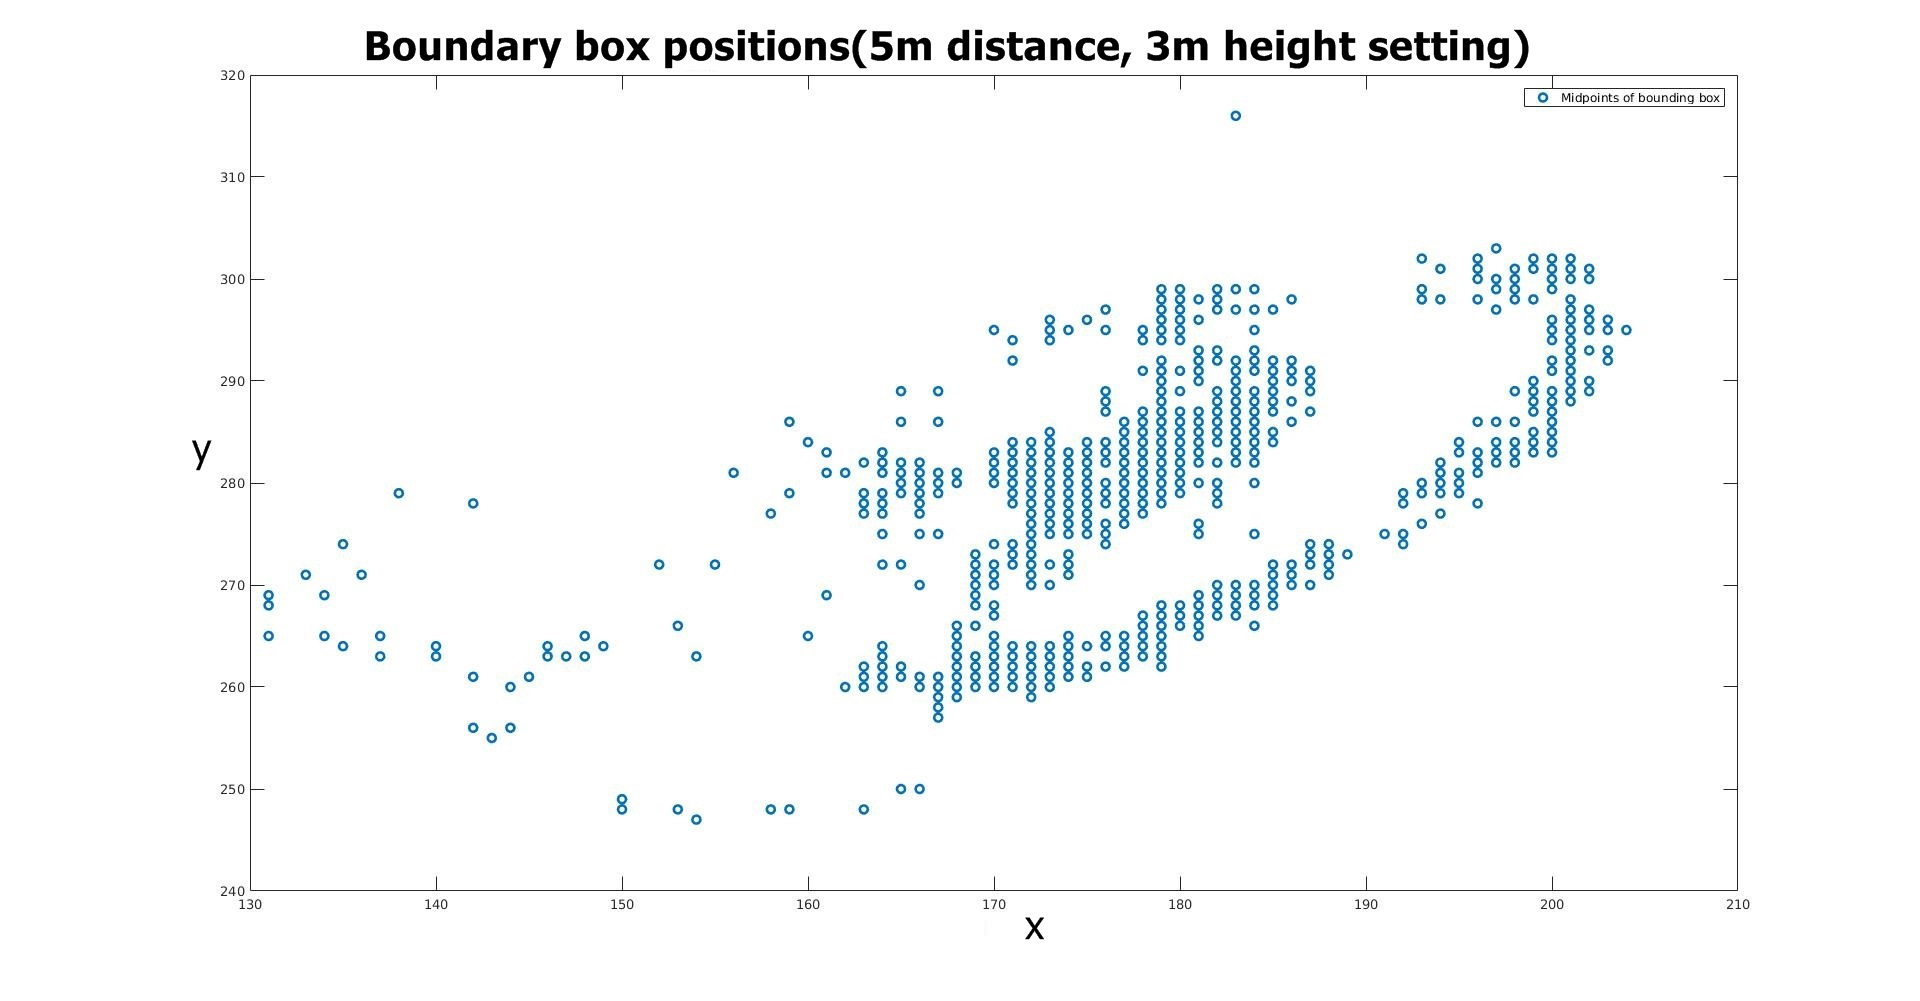
\includegraphics[width=15cm]{bounding_box_positions_d5m_h3m.jpg}
	\caption{Bounding box positions for 5m distance, 3m height\label{Bounding box positions for 5m distance, 3m height}}
\end{figure}

The confidence vs time graph shows the confidence level lies between 0.5 to 0.9.
\begin{figure}[!htb]
	\centering
	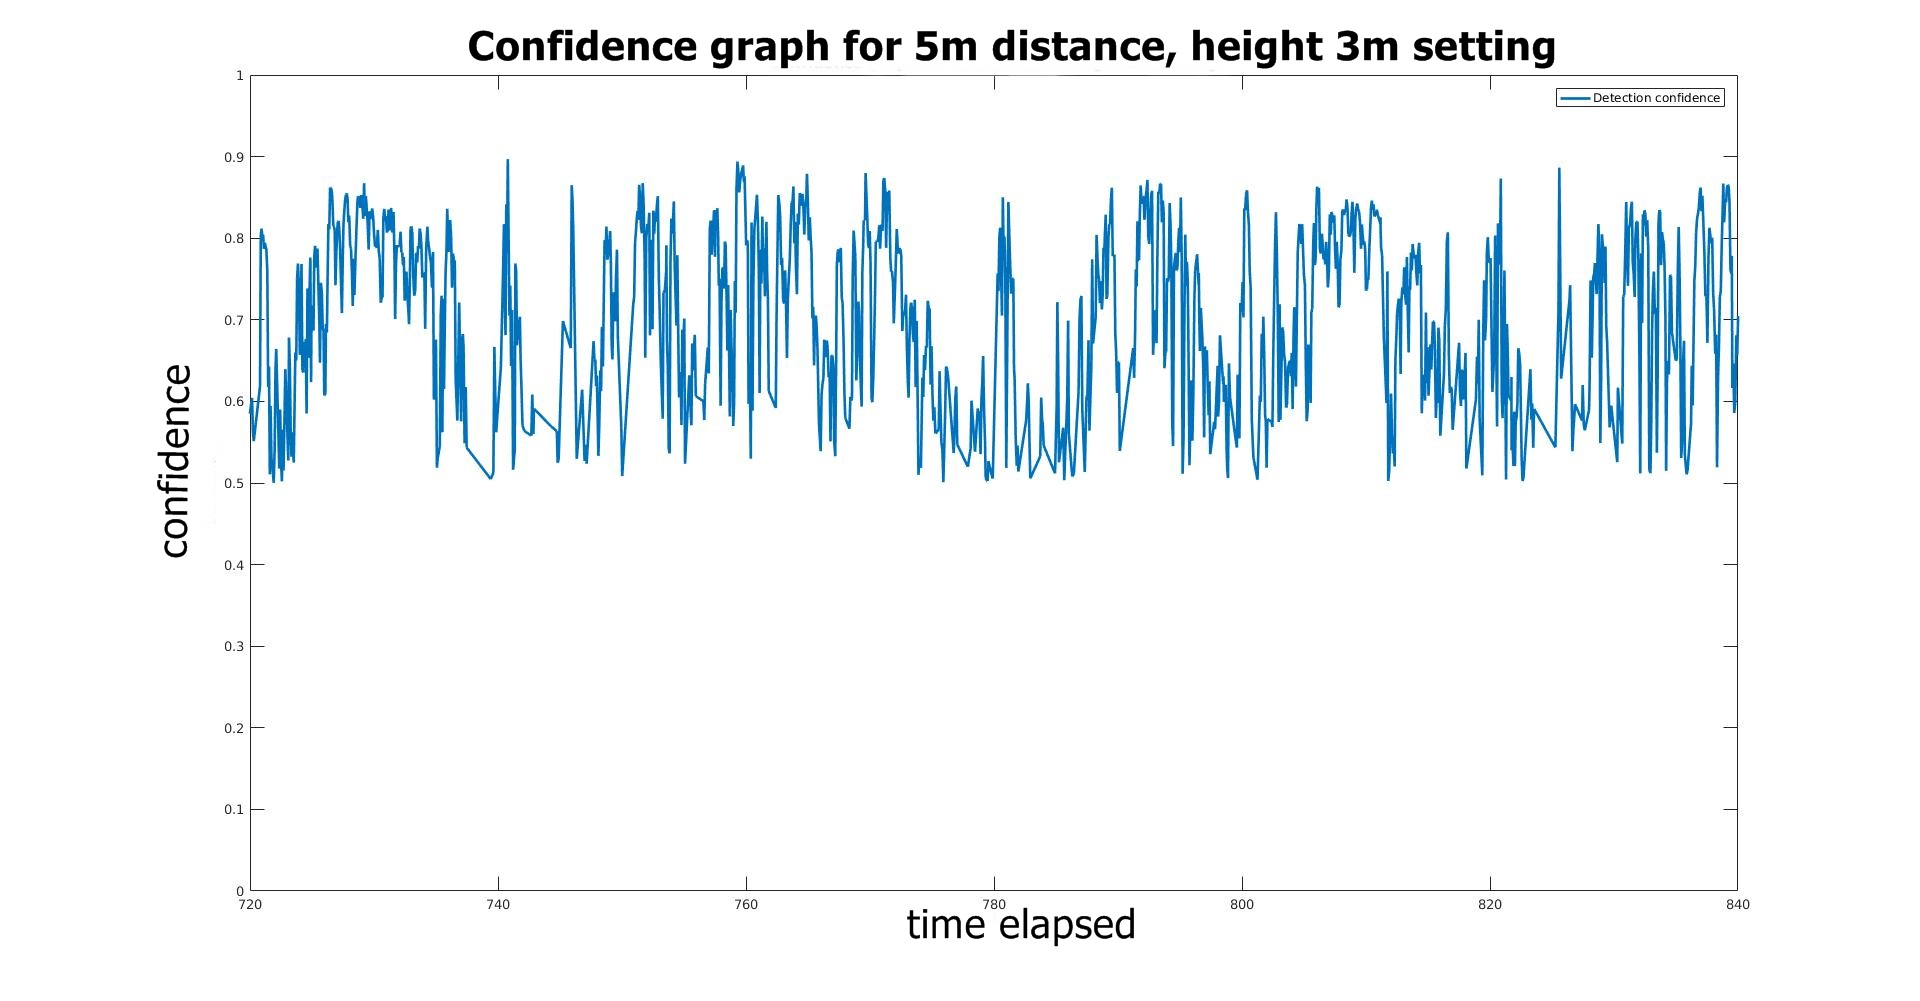
\includegraphics[width=15cm]{confidence_graph_d5m_h3m.jpg}
	\caption{Confidence graph for 5m distance, 3m height\label{Confidence graph for 5m distance, 3m height}}
\end{figure}

\newpage
\subsubsection{Results for 10m distance, 1.5m height}
The results for 10m distance setting showed some erratic results mainly due to the large distance setting. The quadrotor's yaw control took over in this scenario as the human subject can be seen for a greater field of view.

\begin{figure}[!htb]
	\centering
	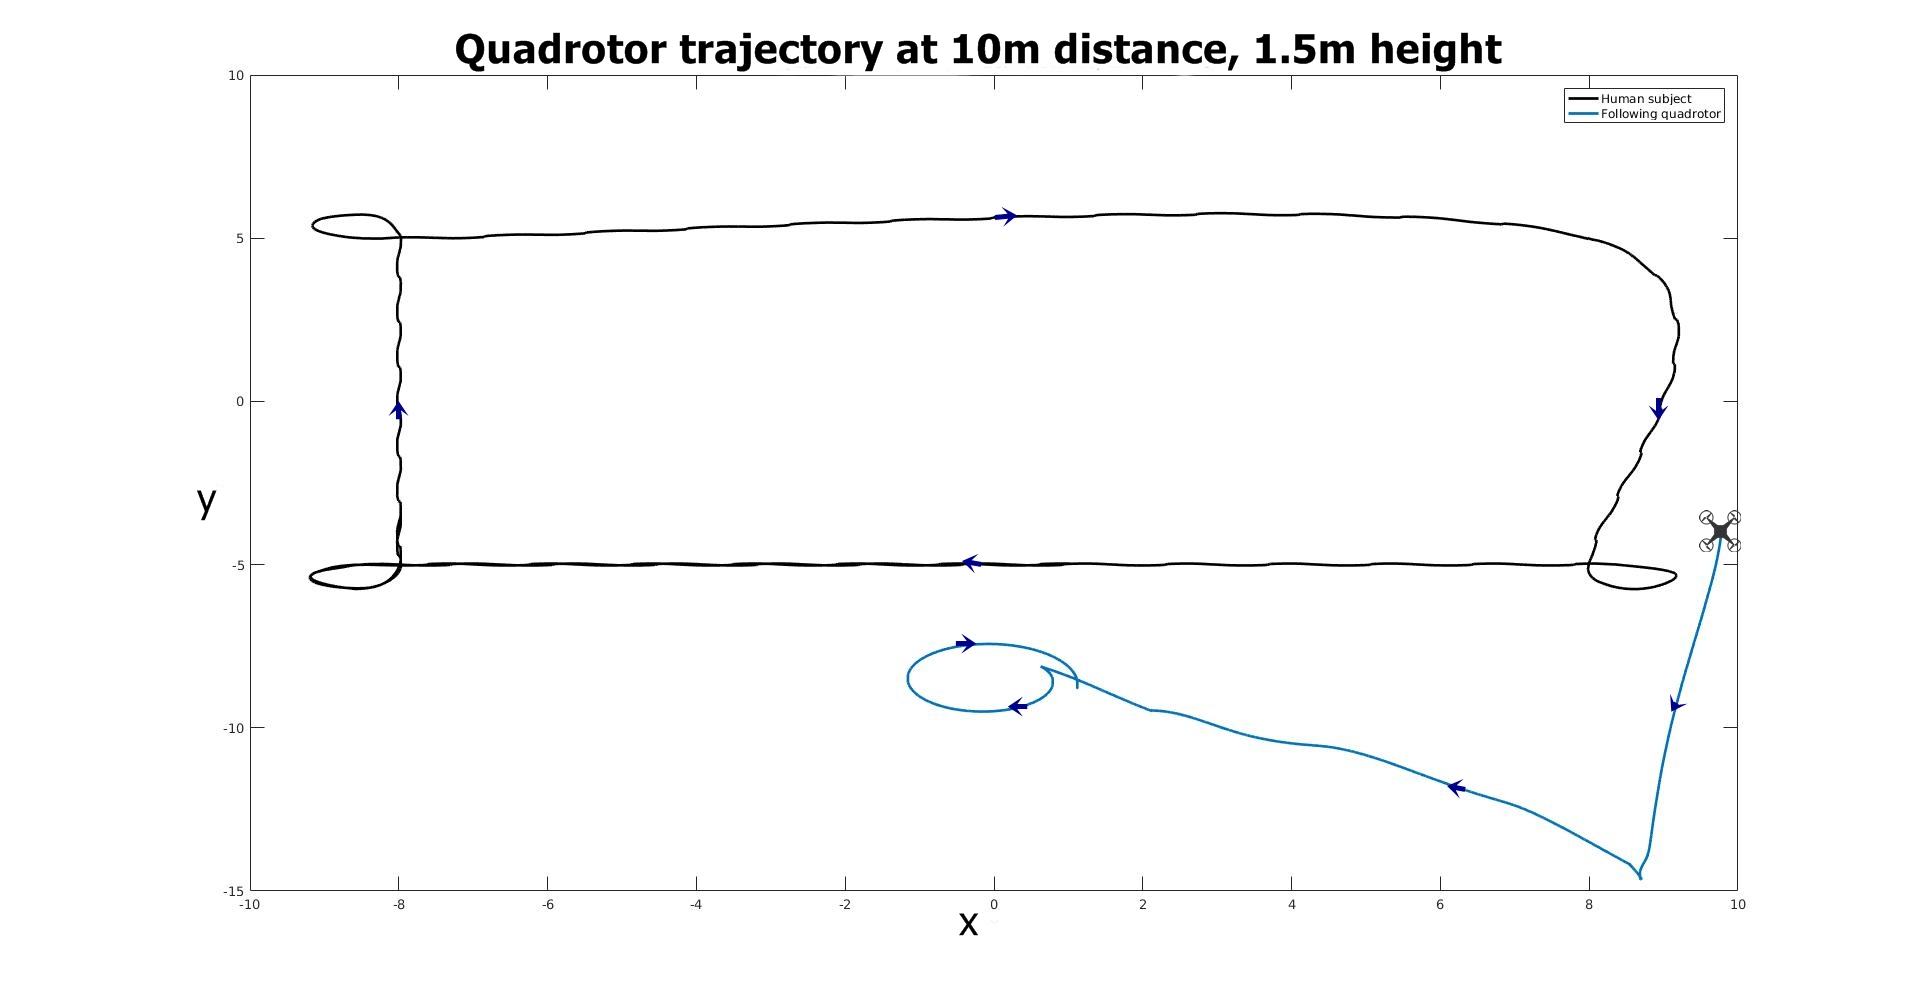
\includegraphics[width=15cm]{quad_path_for_10m_distance.jpg}
	\caption{Quadrotor path for 10m distance, 1.5m height\label{Quadrotor path for 10m distance, 1.5m height}}
\end{figure}

The distance vs time graph shows irregular results cause the initial quadrotor position was outside the human trajectory. The quadrotor required some time to start tracking proper track, causing the irregularity.
\begin{figure}[!htb]
	\centering
	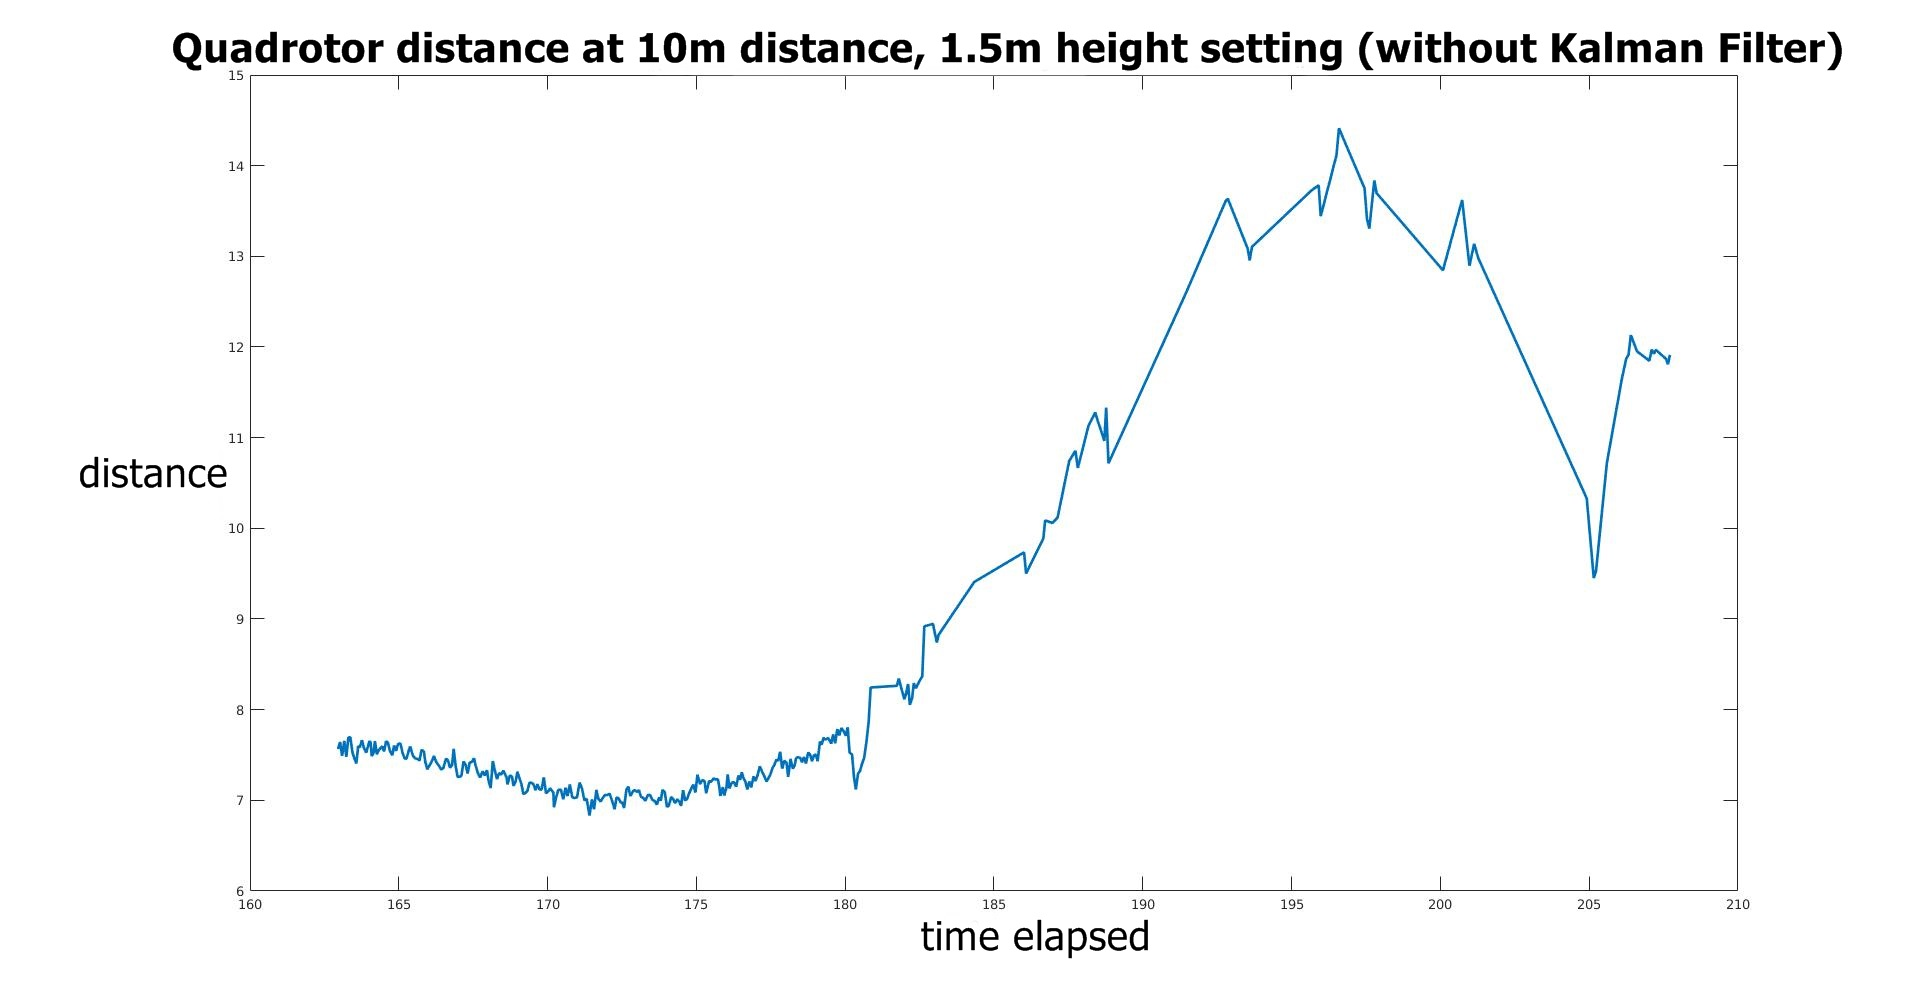
\includegraphics[width=15cm]{distance10m_wokf.jpg}
	\caption{Distance of quadrotor at 10m distance, 1.5m height\label{Distance of quadrotor at 10m distance, 1.5m height}}
\end{figure}

The bounding box graph shows very sparse amount of points within the time frame. This clearly indicates that the detection was very less at this distance setting.
\begin{figure}[!htb]
	\centering
	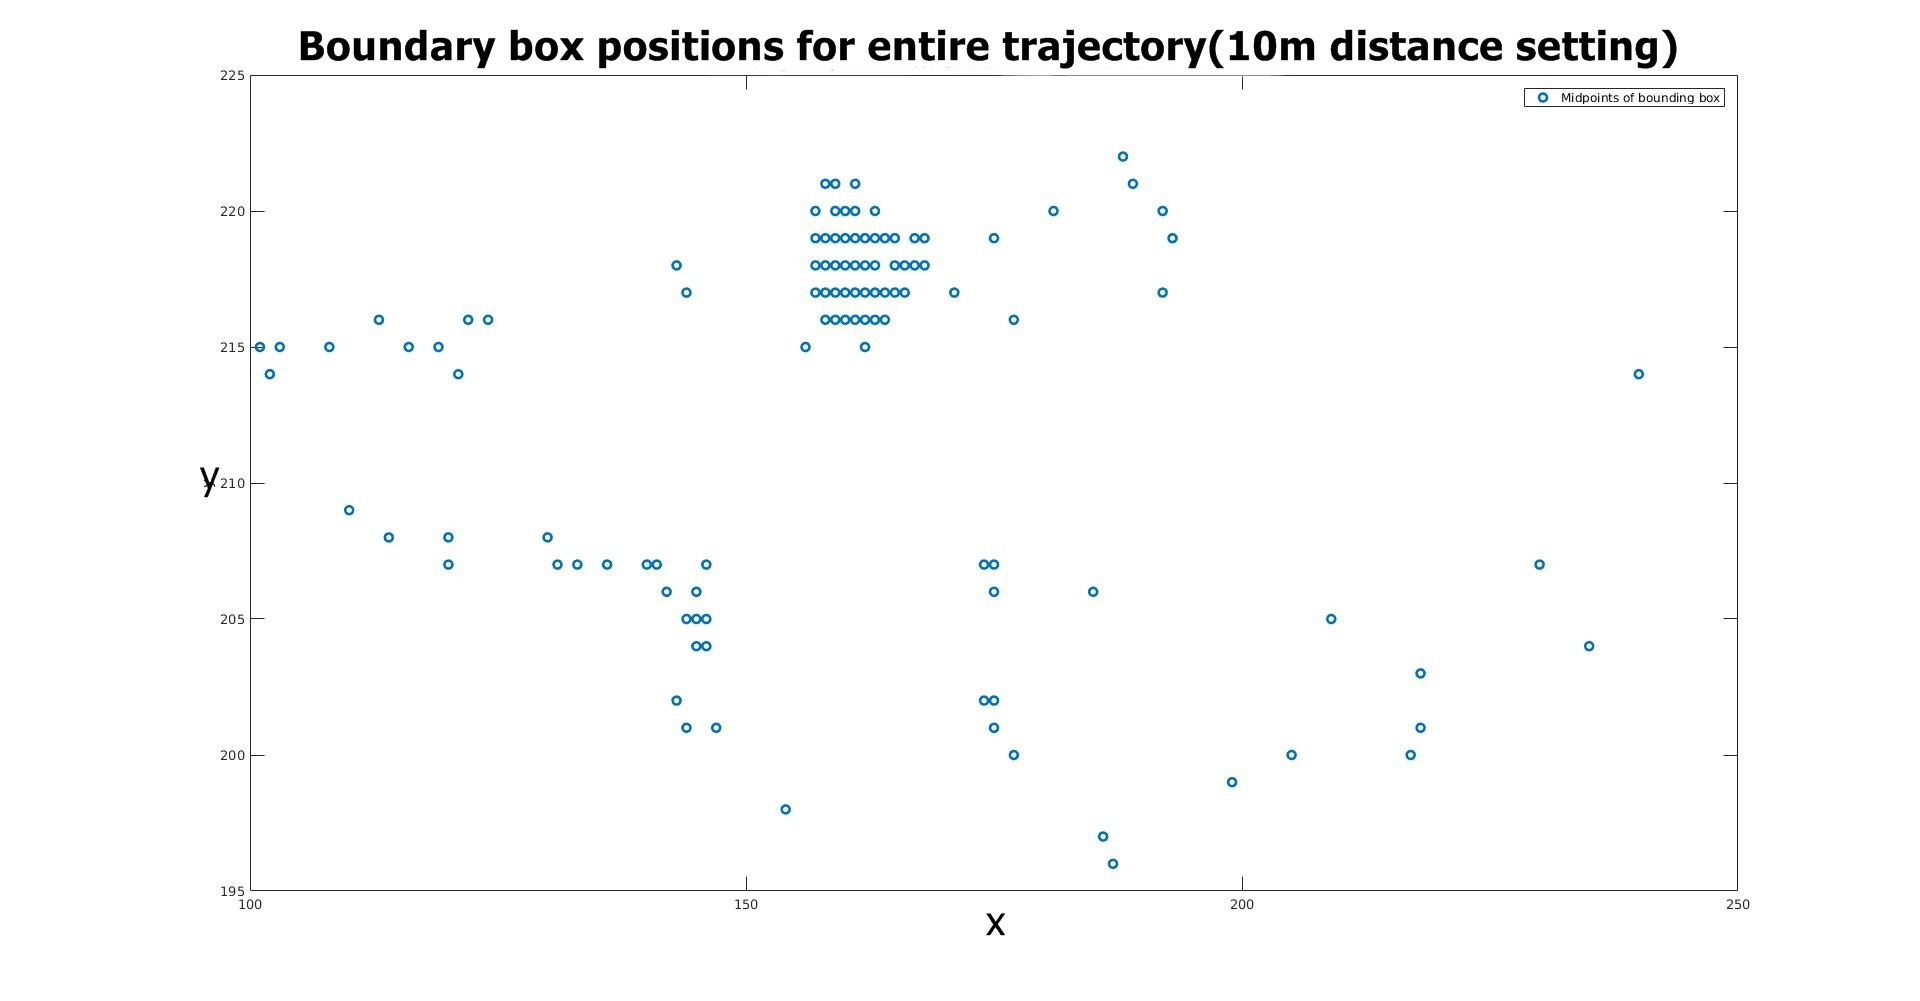
\includegraphics[width=15cm]{bounding_box_positions_10m_distance.jpg}
	\caption{Bounding box positions for 10m distance, 1.5m height\label{Bounding box positions for 10m distance, 1.5m height}}
\end{figure}

The confidence graph also verifies the fact that the detection was very less, causing the jumps and shifts in the graph.
\begin{figure}[!htb]
	\centering
	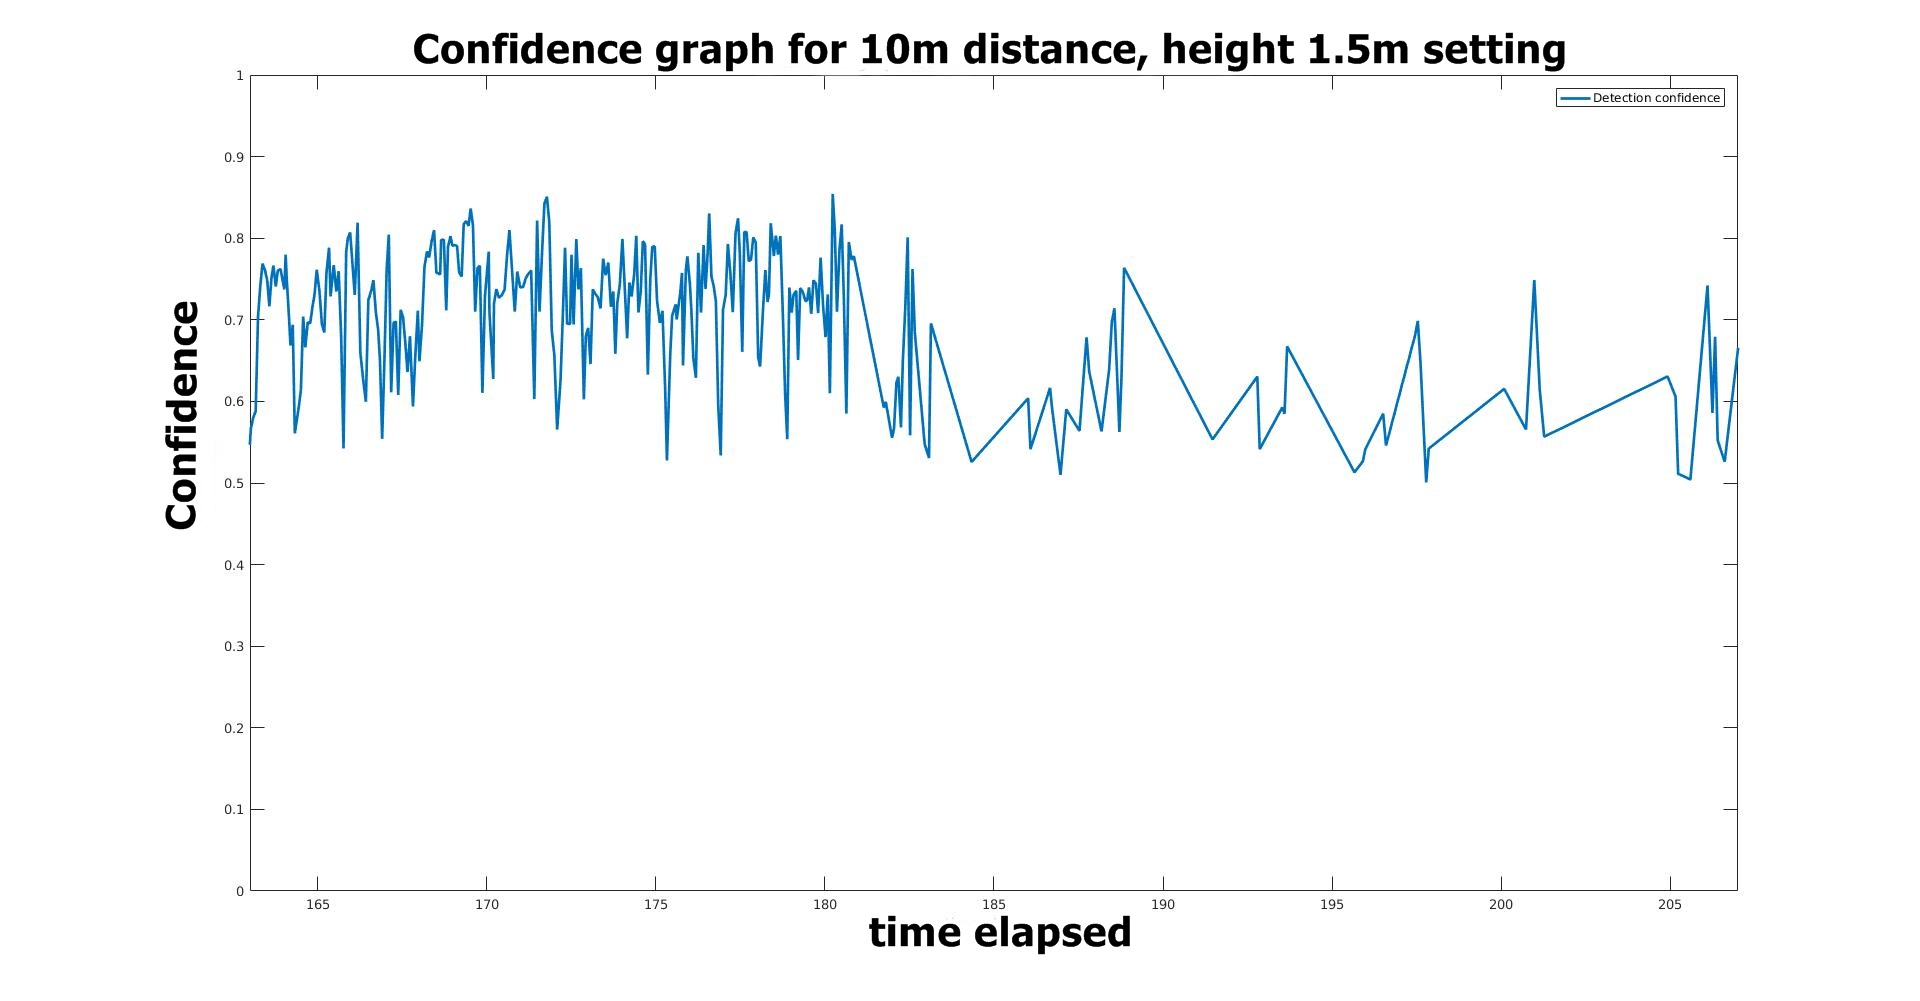
\includegraphics[width=15cm]{confidence_graph_d10m.jpg}
	\caption{Confidence graph for 10m distance, 1.5m height\label{Confidence graph for 10m distance, 1.5m height}}
\end{figure}
Inspite of the meagre amount of detection,the algorithm was able to effectively track the human subject, confirming the feasibility of the method.

\newpage
\subsubsection{Results for different human trajectory path at 3m distance, 2x velocity}
This scenario uses a different path for the human to follow. Note that the sudden changes in the path was ignored by the quadrotor with the help of kalman filter, making a smooth trajectory for itself, while keeping the detection rate intact.

\begin{figure}[!htb]
	\centering
	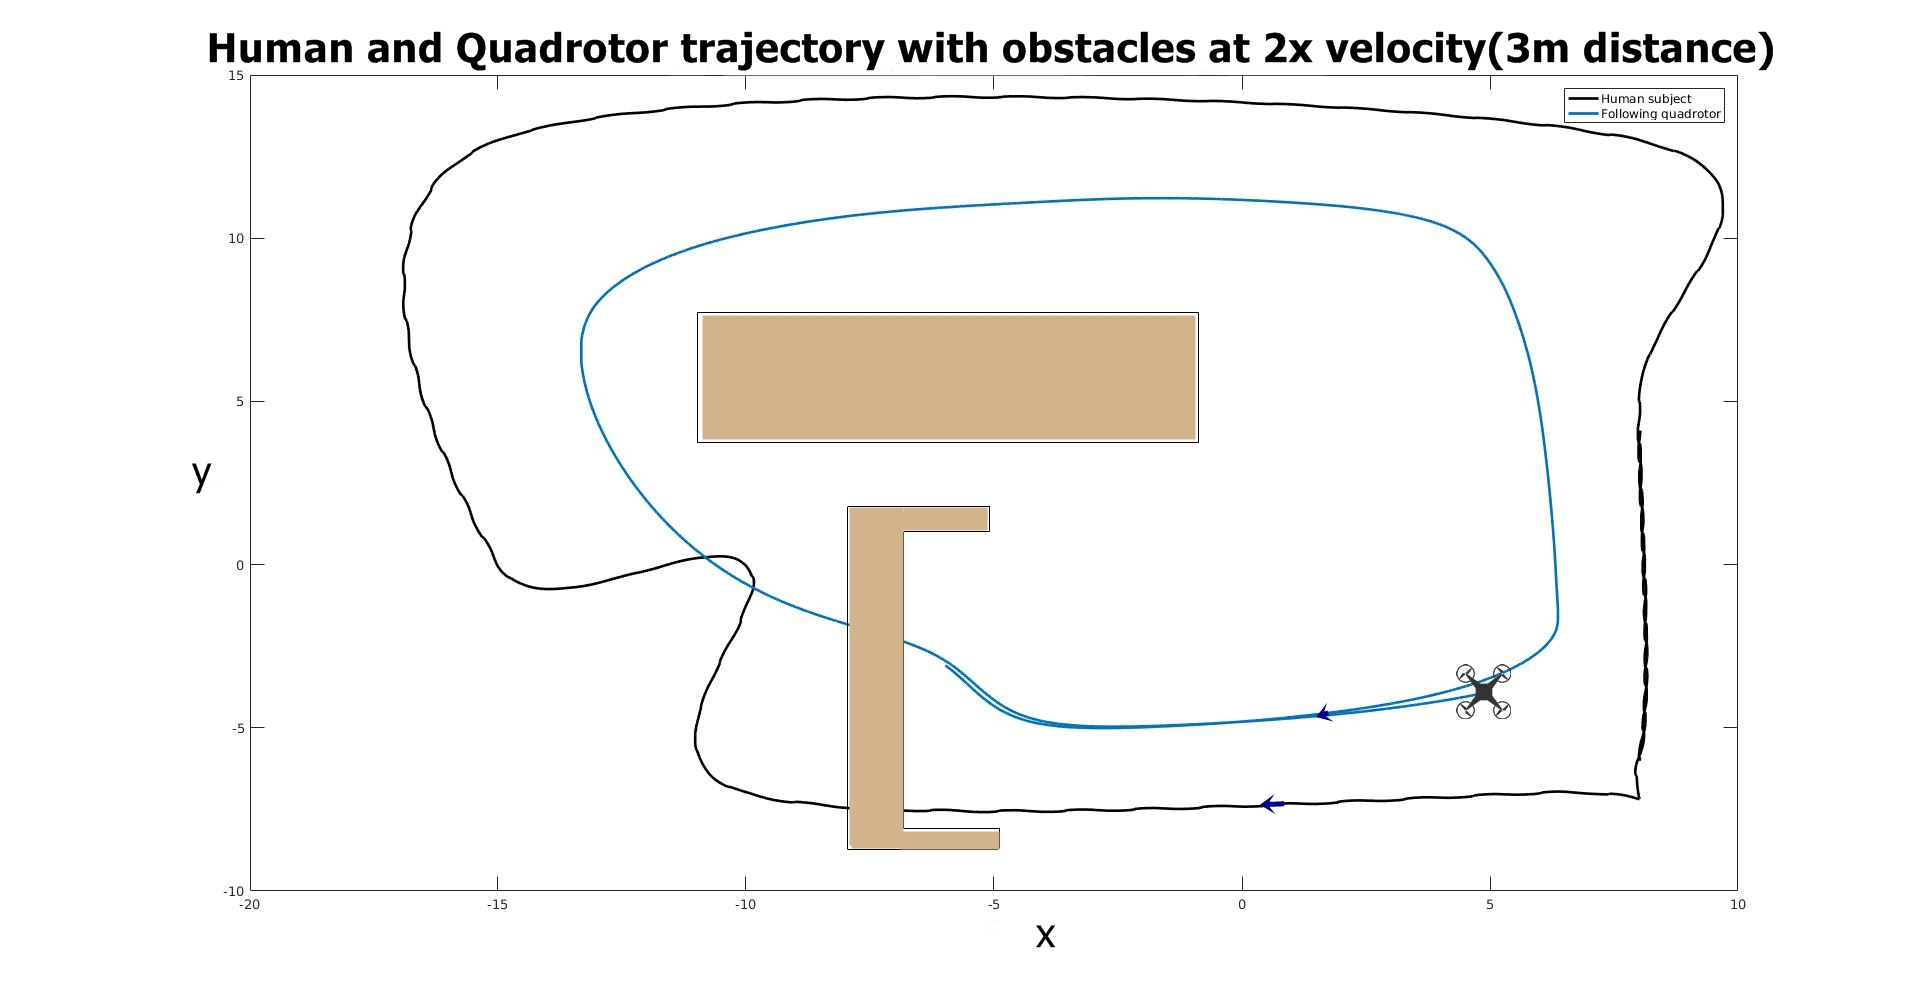
\includegraphics[width=15cm]{quad_path_for_diff_path_2x_velocity_3m_distance.jpg}
	\caption{Quadrotor path for different trajectory, 2x velocity\label{Quadrotor path for different trajectory, 2x velocity}}
\end{figure}

\begin{figure}[!htb]
	\centering
	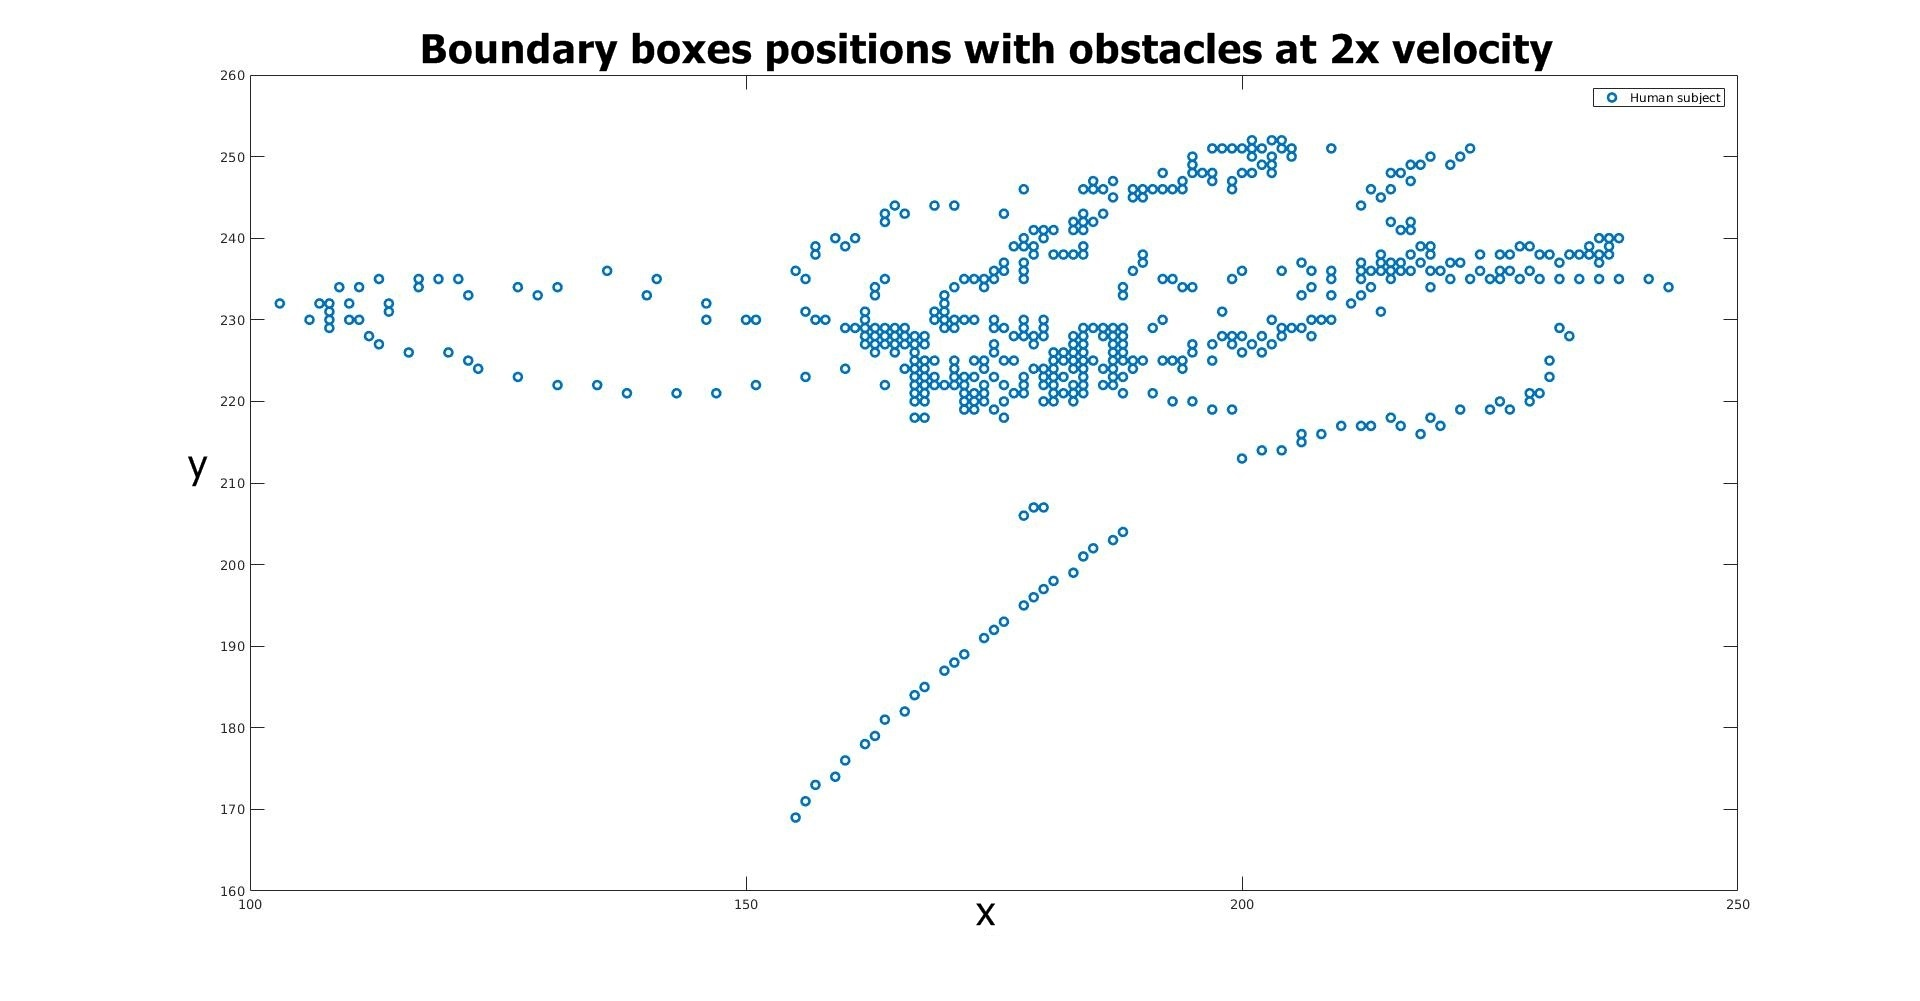
\includegraphics[width=15cm]{bounding_box_positions_diff_path.jpg}
	\caption{Bounding box positions for for different trajectory, 2x velocity\label{Bounding box positions for for different trajectory, 2x velocity}}
\end{figure}





